%-----------------------------------------------------------------------------------------
% Autor dieser Vorlage:
% Stefan Macke (http://fachinformatiker-anwendungsentwicklung.net)
% Permalink zur Vorlage: http://fiae.link/LaTeXVorlageFIAE
%
% Sämtliche verwendeten Abbildungen, Tabellen und Listings stammen von Dirk Grashorn.
%
% Lizenz: Creative Commons 4.0 Namensnennung - Weitergabe unter gleichen Bedingungen
% -----------------------------------------------------------------------------------------

\documentclass[
	ngerman,
	toc=listof, % Abbildungsverzeichnis sowie Tabellenverzeichnis in das Inhaltsverzeichnis aufnehmen
	toc=bibliography, % Literaturverzeichnis in das Inhaltsverzeichnis aufnehmen
	footnotes=multiple, % Trennen von direkt aufeinander folgenden Fußnoten
	parskip=half, % vertikalen Abstand zwischen Absätzen verwenden anstatt horizontale Einrückung von Folgeabsätzen
	numbers=noendperiod % Den letzten Punkt nach einer Nummerierung entfernen (nach DIN 5008)
]{scrartcl}
\pdfminorversion=5 % erlaubt das Einfügen von pdf-Dateien bis Version 1.7, ohne eine Fehlermeldung zu werfen (keine Garantie für fehlerfreies Einbetten!)
\usepackage[utf8]{inputenc} % muss als erstes eingebunden werden, da Meta/Packages ggfs. Sonderzeichen enthalten

% !TEX root = Projektdokumentation.tex

% Hinweis: der Titel muss zum Inhalt des Projekts passen und den zentralen Inhalt des Projekts deutlich herausstellen

\newcommand{\IHKlogo}{logo_handelskammer.png}
\newcommand{\titelOne}{Vereinheitlichung und Digitalisierung}
\newcommand{\titelTwo}{der Materialeingangsprüfungsberichte}
\newcommand{\untertitelOne}{mithilfe einer zentralen Datenbankanbindung}
\newcommand{\untertitelTwo}{im Synchronbereich}
\newcommand{\kompletterTitel}{\titelOne{}\\\titelTwo{}\\\untertitelOne{}\\\untertitelTwo{}}

\newcommand{\amqp}{amqp.png}
\newcommand{\netzplan}{netzplan.png}

\newcommand{\autorName}{Rico Krüger}

\newcommand{\betriebLogo}{logo-bs_sl.png}
\newcommand{\betriebLogoLower}{logo-bs_sl.png}
\newcommand{\betriebName}{Berliner Synchron GmbH}

\newcommand{\betriebAnschrift}{EUREF-Campus 10-11}
\newcommand{\betriebOrt}{10829 Berlin}

\newcommand{\ausbildungsberuf}{Fachinformatiker für Anwendungsentwicklung}
\newcommand{\betreff}{Dokumentation zur betrieblichen Projektarbeit}

\newcommand{\abgabeOrt}{Berlin}
\newcommand{\abgabeTermin}{15.06.2018} % Metadaten zu diesem Dokument (Autor usw.)
% !TEX root = ../Projektdokumentation.tex

% Anpassung an Landessprache ---------------------------------------------------
\usepackage{babel}

% Umlaute ----------------------------------------------------------------------
%   Umlaute/Sonderzeichen wie äüöß direkt im Quelltext verwenden (CodePage).
%   Erlaubt automatische Trennung von Worten mit Umlauten.
% ------------------------------------------------------------------------------
\usepackage[T1]{fontenc}
\usepackage{textcomp} % Euro-Zeichen etc.

% Schrift ----------------------------------------------------------------------
\usepackage{lmodern} % bessere Fonts
\usepackage{relsize} % Schriftgröße relativ festlegen

% Tabellen ---------------------------------------------------------------------
\PassOptionsToPackage{table}{xcolor}
\usepackage{tabularx}
% für lange Tabellen
\usepackage{longtable}
\usepackage{array}
\usepackage{ragged2e}
\usepackage{lscape}
\newcolumntype{w}[1]{>{\raggedleft\hspace{0pt}}p{#1}} % Spaltendefinition rechtsbündig mit definierter Breite

% Grafiken ---------------------------------------------------------------------
\usepackage[dvips,final]{graphicx} % Einbinden von JPG-Grafiken ermöglichen
\usepackage{graphics} % keepaspectratio
\usepackage{floatflt} % zum Umfließen von Bildern
\graphicspath{{Bilder/}} % hier liegen die Bilder des Dokuments

% Sonstiges --------------------------------------------------------------------
\usepackage[titles]{tocloft} % Inhaltsverzeichnis DIN 5008 gerecht einrücken
\usepackage{amsmath,amsfonts} % Befehle aus AMSTeX für mathematische Symbole
\usepackage{enumitem} % anpassbare Enumerates/Itemizes
\usepackage{xspace} % sorgt dafür, dass Leerzeichen hinter parameterlosen Makros nicht als Makroendezeichen interpretiert werden

\usepackage{makeidx} % für Index-Ausgabe mit \printindex
\usepackage[printonlyused]{acronym} % es werden nur benutzte Definitionen aufgelistet

% Einfache Definition der Zeilenabstände und Seitenränder etc.
\usepackage{setspace}
\usepackage{geometry}

% Symbolverzeichnis
\usepackage[intoc]{nomencl}
\let\abbrev\nomenclature
\renewcommand{\nomname}{Abkürzungsverzeichnis}
\setlength{\nomlabelwidth}{.25\hsize}
\renewcommand{\nomlabel}[1]{#1 \dotfill}
\setlength{\nomitemsep}{-\parsep}

\usepackage{varioref} % Elegantere Verweise. „auf der nächsten Seite“
\usepackage{url} % URL verlinken, lange URLs umbrechen etc.

\usepackage{chngcntr} % fortlaufendes Durchnummerieren der Fußnoten
% \usepackage[perpage]{footmisc} % Alternative: Nummerierung der Fußnoten auf jeder Seite neu

\usepackage{ifthen} % bei der Definition eigener Befehle benötigt
\usepackage{todonotes} % definiert u.a. die Befehle \todo und \listoftodos
\usepackage[square]{natbib} % wichtig für korrekte Zitierweise

% PDF-Optionen -----------------------------------------------------------------
\usepackage{pdfpages}
\pdfminorversion=5 % erlaubt das Einfügen von pdf-Dateien bis Version 1.7, ohne eine Fehlermeldung zu werfen (keine Garantie für fehlerfreies Einbetten!)
\usepackage[
    bookmarks,
    bookmarksnumbered,
    bookmarksopen=true,
    bookmarksopenlevel=1,
    colorlinks=true,
% diese Farbdefinitionen zeichnen Links im PDF farblich aus
    linkcolor=bsgrot, % einfache interne Verknüpfungen
    anchorcolor=bsgrot,% Ankertext
    citecolor=bsgrot, % Verweise auf Literaturverzeichniseinträge im Text
    filecolor=bsgrot, % Verknüpfungen, die lokale Dateien öffnen
    menucolor=bsgrot, % Acrobat-Menüpunkte
    urlcolor=bsgrot,
% diese Farbdefinitionen sollten für den Druck verwendet werden (alles schwarz)
    %linkcolor=black, % einfache interne Verknüpfungen
    %anchorcolor=black, % Ankertext
    %citecolor=black, % Verweise auf Literaturverzeichniseinträge im Text
    %filecolor=black, % Verknüpfungen, die lokale Dateien öffnen
    %menucolor=black, % Acrobat-Menüpunkte
    %urlcolor=black,
%
    %backref, % Quellen werden zurück auf ihre Zitate verlinkt
    pdftex,
    plainpages=false, % zur korrekten Erstellung der Bookmarks
    pdfpagelabels=true, % zur korrekten Erstellung der Bookmarks
    hypertexnames=false, % zur korrekten Erstellung der Bookmarks
    linktocpage % Seitenzahlen anstatt Text im Inhaltsverzeichnis verlinken
]{hyperref}
% Befehle, die Umlaute ausgeben, führen zu Fehlern, wenn sie hyperref als Optionen übergeben werden
\hypersetup{
    pdftitle={\titelOne{} \titelTwo{} -- \untertitelOne{} \untertitelTwo},
    pdfauthor={\autorName},
    pdfcreator={\autorName},
    pdfsubject={\titelOne{} \titelTwo{} -- \untertitelOne{} \untertitelTwo},
    pdfkeywords={\titelOne{} \titelTwo{} -- \untertitelOne{} \untertitelTwo},
}


% zum Einbinden von Programmcode -----------------------------------------------
\usepackage{listings}
\usepackage{xcolor}
\definecolor{hellgelb}{rgb}{1,1,0.9}
\definecolor{colKeys}{rgb}{0,0,1}
\definecolor{colIdentifier}{rgb}{0,0,0}
\definecolor{colComments}{rgb}{0,0.5,0}
\definecolor{colString}{rgb}{1,0,0}
\lstset{
    float=hbp,
    basicstyle=\footnotesize,
    identifierstyle=\color{colIdentifier},
    keywordstyle=\color{colKeys},
    stringstyle=\color{colString},
    commentstyle=\color{colComments},
    backgroundcolor=\color{hellgelb},
    columns=flexible,
    tabsize=2,
    frame=single,
    extendedchars=true,
    showspaces=false,
    showstringspaces=false,
    numbers=left,
    numberstyle=\tiny,
    breaklines=true,
    breakautoindent=true,
	captionpos=b,
}
\lstdefinelanguage{cs}{
	sensitive=false,
	morecomment=[l]{//},
	morecomment=[s]{/*}{*/},
	morestring=[b]",
	morekeywords={
		abstract,event,new,struct,as,explicit,null,switch
		base,extern,object,this,bool,false,operator,throw,
		break,finally,out,true,byte,fixed,override,try,
		case,float,params,typeof,catch,for,private,uint,
		char,foreach,protected,ulong,checked,goto,public,unchecked,
		class,if,readonly,unsafe,const,implicit,ref,ushort,
		continue,in,return,using,decimal,int,sbyte,virtual,
		default,interface,sealed,volatile,delegate,internal,short,void,
		do,is,sizeof,while,double,lock,stackalloc,
		else,long,static,enum,namespace,string},
}
\lstdefinelanguage{natural}{
	sensitive=false,
	morecomment=[l]{/*},
	morestring=[b]",
	morestring=[b]',
	alsodigit={-,*},
	morekeywords={
		DEFINE,DATA,LOCAL,END-DEFINE,WRITE,CALLNAT,PARAMETER,USING,
		IF,NOT,END-IF,ON,*ERROR-NR,ERROR,END-ERROR,ESCAPE,ROUTINE,
		PERFORM,SUBROUTINE,END-SUBROUTINE,CONST,END-FOR,END,FOR,RESIZE,
		ARRAY,TO,BY,VALUE,RESET,COMPRESS,INTO,EQ},
}
\lstdefinelanguage{php}{
	sensitive=false,
	morecomment=[l]{/*},
	morestring=[b]",
	morestring=[b]',
	alsodigit={-,*},
	morekeywords={
		abstract,and,array,as,break,case,catch,cfunction,class,clone,const,
		continue,declare,default,do,else,elseif,enddeclare,endfor,endforeach,
		endif,endswitch,endwhile,extends,final,for,foreach,function,global,
		goto,if,implements,interface,instanceof,namespace,new,old_function,or,
		private,protected,public,static,switch,throw,try,use,var,while,xor
		die,echo,empty,exit,eval,include,include_once,isset,list,require,
		require_once,return,print,unset},
}

% fix errors
\usepackage{scrhack} % verwendete Packages
% !TEX root = ../Projektdokumentation.tex

% Seitenränder -----------------------------------------------------------------
\setlength{\topskip}{\ht\strutbox} % behebt Warnung von geometry
\geometry{a4paper,left=20mm,right=20mm,top=25mm,bottom=35mm}

\usepackage[
	automark, % Kapitelangaben in Kopfzeile automatisch erstellen
	headsepline, % Trennlinie unter Kopfzeile
	ilines % Trennlinie linksbündig ausrichten
]{scrpage2}

% Kopf- und Fußzeilen ----------------------------------------------------------
\pagestyle{scrheadings}
% chapterpagestyle gibt es nicht in scrartcl
%\renewcommand{\chapterpagestyle}{scrheadings}
\clearscrheadfoot

% Kopfzeile
\renewcommand{\headfont}{\normalfont} % Schriftform der Kopfzeile
\ihead{\normalsize{\textsc{\titelOne{}\\ \titelTwo}}\\\small{\untertitelOne{} \untertitelTwo}\\[1ex]\textit{\headmark}}
\chead{}
\ohead{\includegraphics[scale=0.05]{\betriebLogoLower}}
\setlength{\headheight}{18mm} % Höhe der Kopfzeile
%\setheadwidth[0pt]{textwithmarginpar} % Kopfzeile über den Text hinaus verbreitern (falls Logo den Text überdeckt)

% Fußzeile
\ifoot{\autorName}
\cfoot{}
\ofoot{\pagemark}

% Überschriften nach DIN 5008 in einer Fluchtlinie
% ------------------------------------------------------------------------------

% Abstand zwischen Nummerierung und Überschrift definieren
% > Schön wäre hier die dynamische Berechnung des Abstandes in Abhängigkeit
% > der Verschachtelungstiefe des Inhaltsverzeichnisses
\newcommand{\headingSpace}{1.5cm}

% Abschnittsüberschriften im selben Stil wie beim Inhaltsverzeichnis einrücken
\renewcommand*{\othersectionlevelsformat}[3]{
  \makebox[\headingSpace][l]{#3\autodot}
}

% Für die Einrückung wird das Paket tocloft benötigt
%\cftsetindents{chapter}{0.0cm}{\headingSpace}
\cftsetindents{section}{0.0cm}{\headingSpace}
\cftsetindents{subsection}{0.0cm}{\headingSpace}
\cftsetindents{subsubsection}{0.0cm}{\headingSpace}
\cftsetindents{figure}{0.0cm}{\headingSpace}
\cftsetindents{table}{0.0cm}{\headingSpace}


% Allgemeines
% ------------------------------------------------------------------------------

\onehalfspacing % Zeilenabstand 1,5 Zeilen
\frenchspacing % erzeugt ein wenig mehr Platz hinter einem Punkt

% Schusterjungen und Hurenkinder vermeiden
\clubpenalty = 10000
\widowpenalty = 10000
\displaywidowpenalty = 10000

% Quellcode-Ausgabe formatieren
\lstset{numbers=left, numberstyle=\tiny, numbersep=5pt, breaklines=true}
\lstset{emph={square}, emphstyle=\color{red}, emph={[2]root,base}, emphstyle={[2]\color{blue}}}

\counterwithout{footnote}{section} % Fußnoten fortlaufend durchnummerieren
\setcounter{tocdepth}{\subsubsectionlevel} % im Inhaltsverzeichnis werden die Kapitel bis zum Level der subsubsection übernommen
\setcounter{secnumdepth}{\subsubsectionlevel} % Kapitel bis zum Level der subsubsection werden nummeriert

% Aufzählungen anpassen
\renewcommand{\labelenumi}{\arabic{enumi}.}
\renewcommand{\labelenumii}{\arabic{enumi}.\arabic{enumii}.}
\renewcommand{\labelenumiii}{\arabic{enumi}.\arabic{enumii}.\arabic{enumiii}}

% Tabellenfärbung:
\definecolor{heading}{rgb}{0.64,0.78,0.86}
\definecolor{odd}{rgb}{0.9,0.9,0.9}
 % Definitionen zum Aussehen der Seiten
% Tabellen, die den Zwischenstand nach einer Projektphase verdeutlichen
\newcommand{\Zwischenstand}[2]{\subsection{Zwischenstand}Tabelle~\ref{tab:#2} zeigt den Zwischenstand nach der #1.\tabelle{Zwischenstand nach der #1}{tab:#2}{#2.tex}}

% Abkürzungen
\newcommand{\Versis}{\textsc{Versis}\xspace}
\newcommand{\NI}{NatInfo\xspace}
\newcommand{\AO}{\textsc{Alte Oldenburger} Krankenversicherung\xspace}
 % eigene allgemeine Befehle, die z.B. die Arbeit mit LaTeX erleichtern
% Tabellen, die den Zwischenstand nach einer Projektphase verdeutlichen
\newcommand{\Zwischenstand}[2]{\subsection{Zwischenstand}Tabelle~\ref{tab:#2} zeigt den Zwischenstand nach der #1.\tabelle{Zwischenstand nach der #1}{tab:#2}{#2.tex}}

% Abkürzungen
\newcommand{\Versis}{\textsc{Versis}\xspace}
\newcommand{\NI}{NatInfo\xspace}
\newcommand{\AO}{\textsc{Alte Oldenburger} Krankenversicherung\xspace}
 % eigene projektspezifische Befehle, z.B. Abkürzungen usw.



\begin{document}

% \phantomsection
% \thispagestyle{empty}
% \pdfbookmark[1]{Eidesstattliche Erklärung}{ihkdeckblatt}
% \includegraphicsKeepAspectRatio{DeckblattIHK}{1}
% \cleardoublepage

\phantomsection
\thispagestyle{plain}
\pdfbookmark[1]{Deckblatt}{deckblatt}
% !TEX root = Projektdokumentation.tex
\begin{titlepage}

\begin{center}
\includegraphics[scale=0.25]{\IHKlogo}\\[1ex]
Abschlussprüfung Sommer 2018 / 2019\\[1ex]
\Large{\ausbildungsberuf}\\
\LARGE{\betreff}\\[1.5ex]
\huge{\textbf{\titelOne\\\titelTwo}}\\
\Large{\textbf{\untertitelOne}}\\
\Large{\textbf{\untertitelTwo}}\\[4ex]

\normalsize
\textbf{Auszubildender:}\\
\autorName\\
Beermannstr. 18\\
12435 Berlin\\[7ex]

\includegraphics[scale=0.07]{\betriebLogo}\\[1.5ex]
\textbf{Ausbildungsstätte}\\
\betriebName{}\\
\betriebAnschrift{}\\
\betriebOrt\\[9ex]

\textbf{Abgabetermin:}\\
\abgabeOrt{}, den \abgabeTermin\\[10ex]

\end{center}

\small
\noindent
Dieses Werk, einschließlich seiner Teile, ist \textbf{urheberrechtlich geschützt}.
Jede Verwertung außerhalb der engen Grenzen des Urheberrechtsgesetzes ist ohne Zustimmung des Autors unzulässig und strafbar.
Das gilt insbesondere für Vervielfältigungen, Übersetzungen sowie die Einspeicherung und Verarbeitung in elektronischen Systemen.

\end{titlepage}

\cleardoublepage

% Preface --------------------------------------------------------------------
\phantomsection
\pagenumbering{Roman}
\pdfbookmark[1]{Inhaltsverzeichnis}{inhalt}
\tableofcontents
\cleardoublepage

\phantomsection
\listoffigures
\cleardoublepage

\phantomsection
\listoftables
\cleardoublepage

\phantomsection
\lstlistoflistings
\cleardoublepage

\newcommand{\abkvz}{Abkürzungsverzeichnis}
\renewcommand{\nomname}{\abkvz}
\section*{\abkvz}
\markboth{\abkvz}{\abkvz}
\addcontentsline{toc}{section}{\abkvz}
% !TEX root = Projektdokumentation.tex

% Es werden nur die Abkürzungen aufgelistet, die mit \ac definiert und auch benutzt wurden. 
%
% \acro{VERSIS}{Versicherungsinformationssystem\acroextra{ (Bestandsführungssystem)}}
% Ergibt in der Liste: VERSIS Versicherungsinformationssystem (Bestandsführungssystem)
% Im Text aber: \ac{VERSIS} -> Versicherungsinformationssystem (VERSIS)

% Hinweis: allgemein bekannte Abkürzungen wie z.B. bzw. u.a. müssen nicht ins Abkürzungsverzeichnis aufgenommen werden
% Hinweis: allgemein bekannte IT-Begriffe wie Datenbank oder Programmiersprache müssen nicht erläutert werden,
%          aber ggfs. Fachbegriffe aus der Domäne des Prüflings (z.B. Versicherung)

% Die Option (in den eckigen Klammern) enthält das längste Label oder
% einen Platzhalter der die Breite der linken Spalte bestimmt.
\begin{acronym}[WWWWWW]
	\acro{IHK}{Industrie- und Handelskammer}
	\acro{BSG}{Berliner Synchron GmbH}
	\acro{MEP}{Materialeingangsprüfungsbericht}
	\acro{QC}{Quality Check}
	\acro{Ruby}{Objektorientierte Programmiersprache}
	\acro{Framework}{Programmiergerüst}
	\acro{Rails}{\acs{Framework} für Webanwendungen}
	\acro{RoR}{\acs{Ruby} on \acs{Rails}}
	\acro{SQL}{Structured Query Language: Programmiersprache für Datenbankabfrage}
	\acro{MySQL}{My Structured Query Language: Relationale Datenbank}
	\acro{HTTP}{Hypertext Transfer Protocol: Protokoll zur Datenübertragung}
	\acro{mysql2}{\acs{MySQL}-Datenbank-Connector}
	\acro{gem}{Bezeichnung für Bibliotheken und Frameworks in Ruby}
	\acro{HTML}{Hypertext Markup Language: Programmiersprache zur Strukturierung einer Webseite}
	\acro{HAML}{\acs{HTML} abstraction markup language: Programmiersprache zur Generierung von HTML-Code; Erlaubt u.a.\ die Ausführung von Ruby-Code}
	\acro{CSS}{Cascading Style Sheets: Programmiersprache zum Designen von Webseiten}
	\acro{Javascript}{Scriptsprache zum Erstellen dynamischer Webseiten}
	\acro{Bootstrap}{\acs{HTML}-, \acs{CSS}-, \acs{Javascript}-\acs{Framework}}
	\acro{Model}{Datenmodel}
	\acro{View}{Darstellung}
	\acro{Controller}{Programmsteuerung}
    \acro{MVC}{\acs{Model}-\acs{View}-\acs{Controller}: Architekturdesign zur Trennung der Software in drei Komponenten: \acs{Model}, \acs{View} und \acs{Controller}}
    \acro{CRUD}{Create Read Update Delete}
    \acro{GUI}{Graphical User Interface}
    \acro{rvm}{Ruby Version Manager}
    \acro{IDE}{Integrated Development Envrionment}
    
	

\end{acronym}

\clearpage

% Inhalt ---------------------------------------------------------------------
\pagenumbering{arabic}
% !TEX root = Projektdokumentation.tex
% !TEX root = ../Projektdokumentation.tex

\nocite{*}
\section{Einleitung}
\label{sec:Einleitung}
% TODO: Zitat finden, in dem es um den Wert der eigenständigen Projektarbeit geht, und dann hier einfügen.
\subsection{Projektumfeld} 
\label{sec:Projektumfeld}
% Kurze Vorstellung des Ausbildungsbetriebs (Geschäftsfeld, Mitarbeiterzahl \usw)
\paragraph*{Ausbildungsbetrieb: } Die \ac{BSG} ist ein mittelständisches, international agierendes Unternehmen, dessen Kerngebiet die deutsche Synchronisation englischsprachiger Filme und Serien ist. 1949 als erstes Synchronunternehmen Deutschlands gegründet, hält die \ac{BSG} nach wie vor eine Spitzenstellung innerhalb der Synchronbranche. Seit 2016 ist das Unternehmen Teil der S\&L Medien Gruppe GmbH, die es sich zum Ziel gesetzt hat, ein allumfassendes Unterhaltungsmarketing zu bieten. Neben den rund 60 festen Mitarbeitern, greift die \ac{BSG} auf einen Pool aus über 3 000 Synchronschauspielern, Autoren, Regisseuren, Cuttern und Takern zurück. Die interne IT-Abteilung des Unternehmens beschäftigt derzeit eine Vollzeitkraft und einen Auszubildenden. Unterstützt wird diese durch die IT-Abteilung der S\&L Medien Gruppe sowie durch einen technischen Dienstleister vor Ort. Das Aufgabenfeld der IT-Abteilung umfasst den Aufbau und die Wartung des firmeninternen Netzwerks, die Administration der eigenen Server, die Entwicklung und Pflege der in der Firma eingesetzten Systeme sowie die alltägliche Benutzerunterstützung.

% Wer ist Auftraggeber/Kunde des Projekts?
\paragraph*{Auftraggeber: } Der Auftraggeber ist in diesem Projekt der Ausbildungsbetrieb – die \ac{BSG}.

\paragraph*{Projektbeschreibung: }Derzeit befindet sich eine neue Software – Copper in der Testphase. Diese wird von einem externen Dienstleister in Zusammenarbeit mit der \ac{BSG} programmiert. Mit Copper sollen alle Tätigkeiten von der Projekterstellung über die Projektumsetzung bis hin zur Projektauswertung gesteuert und alle betrieblichen Prozesse über ein Webinterface zentralisiert dargestellt werden. Eine zusätzliche Webanwendung soll für die neue Software entwickelt werden. Diese Webanwendung soll ein Eingabeformular für einen \ac{MEP} bereitstellen und die vom Benutzer eingegebenen Daten in eine zentrale Datenbank speichern.

\subsection{Projektziel} 
\label{sec:Projektziel}
% Worum geht es eigentlich?
\paragraph*{Projekthintergrund: } Die Synchronisation von Filmen und Serien wird jeweils als ein Projekt bezeichnet. Die Akte eines Kinofilms bzw. die Episoden einer Serie bilden dabei einzelne Teilprojekte. Um diese Teilprojekte in deutscher Sprache aufzunehmen, erhält die Berliner Synchron GmbH von seinen Kunden, meist ausländische Produktionsstudios, sowohl das zu synchronisierende Video- als auch diverse Audiomaterialien. Dabei handelt es sich um unterschiedliche Audiotypen wie Originalton, Musik, Effekte und andere, von denen es wiederum unterschiedliche Versionen gibt. Bevor das gelieferte Material in den Produktionsprozess integriert werden kann, muss dieses analysiert werden. Dabei wird es auf Fehler überprüft und die Qualität des angelieferten Materials wird bewertet. Diese Bewertung kann dazu führen, dass das Audiomaterial überarbeitet oder sogar erneut vom Kunden zugesandt werden muss. Bisher wird das Ergebnis dieser Prüfung formfrei, meist in Word-Dateien, verfasst. Danach werden diese in den entsprechenden Projektordnern gespeichert und die betreffenden Projektbeteiligten per E-Mail informiert.

% Was soll erreicht werden?
\paragraph*{Ziel des Projekts: } Ziel dieses Projektes ist die Entwicklung einer einfachen und leicht bedienbaren Webanwendung zur Erfassung, Darstellung und zentralen Speicherung der Daten der Materialeingangsprüfung und deren direkter Zuordnung zu einem Teilprojekt. Alle Mitarbeiter sollen nach einer kurzen Einführung in der Lage sein, ein solches Formular problemlos ausfüllen zu können.

\subsection{Projektbegründung} 
\label{sec:Projektbegruendung}
% Warum ist das Projekt sinnvoll (\zB Kosten- oder Zeitersparnis, weniger Fehler)?
\paragraph*{Nutzen des Projekts: } Durch ein standardisiertes Formular mit zum Großteil vorgegebenen Werten über Auswahlfeldern soll die Erstellung eines solchen Meldeberichtes erleichtert und damit beschleunigt werden. Das Projekt setzt auf einen weiteren wichtigen Schwerpunkt: dem Controlling. Neben der Kostenerfassung für den Materialeingangsbericht durch Copper, lässt die zentralisierte Erfassung der Daten und die direkte Zuordnung zu den Projekten und Kunden auch eine übersichtliche und gefilterte Darstellung aller \ac{MEP}s zu. Damit lassen sich Rückschlüsse auf anfallende Kosten für zukünftige Projekte ziehen. Schickt ein Kunde regelmäßig fehlerhaftes Material, verzögert sich die Produktion und die Kosten steigen. Das Erstellen eines solchen Berichts ist auf Grund seines Umfangs nicht Teil dieses Projekts und wird erst in einem Nachfolgeprojekt entwickelt. Die Erstellung und Speicherung der Daten eines Materialeingangs stellt lediglich die Grundlage dar.

% Was ist die Motivation hinter dem Projekt?
\paragraph*{Motivation: } Der Auftraggeber ist daran interessiert, ein allumfassendes System für die Projektabwicklung zu haben, welches alle Projektschritte dokumentiert und darstellt. Zu diesem Zweck wurde die Software Copper in Auftrag gegeben. Sie wird von einem externen Dienstleister entwickelt und nach erfolgreicher Einführung von der eigenen IT-Abteilung erweitert werden.

\subsection{Projektschnittstellen} 
\label{sec:Projektschnittstellen}
% Mit welchen anderen Systemen interagiert die Anwendung (technische Schnittstellen)?
Copper ist eine Webapplikation, die mit \ac{RoR} erstellt wurde. Da diese Anwendung später auf einem firmeneigenen Server ausgeführt und hauptsächlich im lokalen Netzwerk eingesetzt wird, soll diese vor allem über den in der \ac{BSG} eingesetzten Webbrowser – Google Chrome\footnote{https://www.google.de/chrome/} ausführbar sein. Zur Erstellung der Webseite wird \acs{Bootstrap} verwendet. Die browserbasierten Nutzereingaben werden dann mittels \acs{HTTP} von einem Apache-Webserver entgegen genommen und an die \acs{Rails}-Applikation übermittelt. Dort werden die Anfragen bearbeitet und beantwortet, sowie ggf.\ in eine lokale \acs{MySQL}-Datenbank geschrieben oder ausgelesen. Die Anwendung ist vor allem für die \ac{QC}-Abteilung im Unternehmen gedacht. Die Verantwortliche der \ac{QC}-Abteilung sowie der Ausbilder sind für die Projektabnahme verantwortlich.

\subsection{Projektabgrenzung} 
\label{sec:Projektabgrenzung}

\paragraph*{Was dieses Projekt nicht bietet: } Eine automatisierte Auswertung sowie sonstige Zusammenfassungen außerhalb eines Teilprojektes werden nicht vorgenommen. Dieses Projekt stellt lediglich die Grundlage dar. Zudem wird die Software während des Projektes noch nicht in Copper integriert. (Siehe  \hyperref[sec:AbweichungenProjektantrag]{Siehe Abweichung vom Projektantrag}).
% !TEX root = ../Projektdokumentation.tex
\section{Projektplanung} 
\label{sec:Projektplanung}
Der Projektplanung ging ein Meeting zwischen der Geschäftsführung, einer Mitarbeiterin, welche zum Großteil Materialeingangsberichte erfasst und der IT-Abteilung voraus. Nachdem die Geschäftsführung sich nach einer Zusammenfassung der Materialeingangsprüfungsberichte für einen bestimmten Kunden erkundigte bzw. nach der Möglichkeit einer solchen, wurde schnell klar, dass dies auf Basis der aktuellen Arbeitsweise nicht gewährleistet werden kann. Für eine übersichtliche, gefilterte Darstellung solcher Berichte würde eine gewisse Standardisierung und zentrale Speicherung der Daten benötigt. Auf dieser Grundlage entstand die Idee eine Erweiterung für Copper zu entwickeln.

\subsection{Projektphasen}
\label{sec:Projektphasen}
% In welchem Zeitraum und unter welchen Rahmenbedingungen (\zB Tagesarbeitszeit) findet das Projekt statt?
Aufgrund des von der \ac{IHK} vorgegebenen begrenzten Zeitrahmens, wurde das Projekt in ein Teilprojekt gewandelt. Nach der positiven Rückmeldung auf meinen Projektantrag wurde das Projekt in den Tagesablauf meiner betrieblichen Arbeit integriert und mit ca. 30 Wochenstunden bearbeitet.

\subsection{Zeitplanung}
\label{sec:Zeitplanung}
% Verfeinerung der Zeitplanung, die bereits im Projektantrag vorgestellt wurde.
Für die Umsetzung des Projektes stehen seitens der Anforderungen der \ac{IHK} 70 Stunden zur Verfügung. Diese wurden zur Antragstellung auf die einzelnen Phasen verteilt. Die grobe Zeitplanung der Hauptphasen kann nachfolgender Tabelle~\ref{tab:Zeitplanung} Zeitplanung entnommen werden. Eine ausführlichere Zeitplanung findet sich im~\Anhang{subsec:Zeitplan}.

\tabelle{Zeitplanung}{tab:Zeitplanung}{ZeitplanungKurz}

\subsection{Abweichungen vom Projektantrag}
\label{sec:AbweichungenProjektantrag}
Bei der Erstellung des Projektantrags wurde geplant, das Projekt auf einer bereits vorhandenen Testumgebung aufzusetzen und in Absprache mit dem Entwickler von Copper anzufertigen. Da der Entwickler von Copper während der Projektarbeit weder erreichbar, noch ein Zugriff auf die Testumgebung vorhanden war, musste das Projekt mit den zur Verfügung stehenden Daten zur Zeit der Erstellung des Projektantrags nachgebaut werden. Somit ergaben sich erhebliche Änderungen im Vergleich zum Projektantrag. Ferner konnte aufgrund der am Ende fehlenden Zeit durch die vorhergehenden, nicht eingeplanten Entwicklungsarbeiten keine automatisierten Tests des entwickelnden Materialeingangsberichts mehr durchgeführt werden. Das hätte das zusätzliche Aufsetzen einer Testumgebung bedurft, welche am Ende nicht einmal den tatsächlichen Produktionseinsatz der Anwendung sichergestellt hätte. Daher wurde in Absprache mit dem Ausbilder beschlossen, lediglich ein Testprotokoll zu erstellen. Weiterhin wurde auf die Erstellung einer Entwicklerdokumentation verzichtet.

\subsection{Ressourcenplanung}
\label{sec:Ressourcenplanung}
% Detaillierte Planung der benötigten Ressourcen (Hard-/Software, Räumlichkeiten \usw).
% \Ggfs sind auch personelle Ressourcen einzuplanen (\zB unterstützende Mitarbeiter).
% Hinweis: Häufig werden hier Ressourcen vergessen, die als selbstverständlich angesehen werden (\zB PC, Büro).
Alle benötigten Ressourcen zur Durchführung des Projekts sind bereits im Unternehmen vorhanden bzw. können online heruntergeladen werden. Eine Auflistung befindet sich im ~\Anhang{app:Ressourcen}.

\subsection{Entwicklungsprozess}
\label{sec:Entwicklungsprozess}
% Welcher Entwicklungsprozess wird bei der Bearbeitung des Projekts verfolgt (\zB Wasserfall, agiler Prozess)?
Die Entwicklung des Projekts  erfolgt nach Rücksprache mit der verantwortlichen Mitarbeiterin für Qualitätsprüfung im Unternehmen. Ansonsten wird das Projekt weitestgehend nach dem Wasserfallmodell in Eigenregie erstellt.

% !TEX root = ../Projektdokumentation.tex
\section{Analysephase} 
\label{sec:Analysephase}
% Überblick
Die erste Analysephase wurde bereits zum Zeitpunkt der Antragstellung des \ac{IHK}-Projektes durchgeführt. Dort wurde bereits mit dem externen Entwickler gesprochen und auf der Grundlage eines Skripts, geschrieben in der Datenbanksprache \acs{SQL}, ein vorläufiges Datenbankmodell für das Projekt erstellt und eingegrenzt.

\subsection{Ist-Analyse} 
\label{sec:IstAnalyse}
% Wie ist die bisherige Situation (\zB bestehende Programme, Wünsche der Mitarbeiter)?
In der \ac{BSG} wird sowohl das eingehende als auch das ausgehende Audio- und Videomaterial analysiert und auf Fehler überprüft. Bei der Analyse werden neben möglichen Fehlern auch Meta-Daten wie das Materialeingangsdatum, Audioformat oder die Version gesammelt. Zudem wird entschieden, ob das Material nochmal überarbeitet oder gar vom Kunden neu übermittelt werden muss, bevor es in die Produktion geht. Eine solche Prüfung wird bisher formlos, meist in Word-Dateien geschrieben. Danach werden die für das Projekt verantwortlichen Mitarbeiter per E-Mail über die Fertigstellung und auf mögliche Mängel hingewiesen. Bei einem solchen Bericht gibt es viele Informationen, welche nur einen begrenzt möglichen Datensatz aufweisen. Weiterhin werden dann die Berichte in den entsprechenden Netzwerkordnern der einzelnen Teilprojekte gespeichert. Das Erhalten eines Überblicks über die Materialeingänge und deren Fehler für ein Teilprojekt ist somit äußerst schwierig. Will man einen solchen Überblick über ein komplettes Projekt oder gar für einen Kunden erhalten, ist dies nahezu unmöglich. Dies erschwert die Kostenberechnung und das Ziehen von Rückschlüssen für künftige Projekte.

\subsection{Wirtschaftlichkeitsanalyse}
\label{sec:Wirtschaftlichkeitsanalyse}
Die Wirtschaftlichkeit des neuen standardisierten Berichts zur Qualitätssicherung steht außer Frage. Die derzeitige Darstellung und Bearbeitung ist unübersichtlich und ineffizient. Die Vielzahl der Erstellung von Berichten würde sich in jedem Fall mittelfristig gesehen, refinanzieren. Mit der Inbetriebnahme der neuen Software sollen zudem alle übrigen Projektprozesse dargestellt und deren Kosten ermittelt werden. Warum also die Erstellung eines solchen Berichts ausschließen? Das würde wiederum das Controlling erschweren und auch für diese Kostenstelle einen zusätzlichen Zeit- und damit Kostenaufwand bedeuten.

\subsubsection{\gqq{Make or Buy}-Entscheidung}
\label{sec:MakeOrBuyEntscheidung}
% Gibt es vielleicht schon ein fertiges Produkt, dass alle Anforderungen des Projekts abdeckt?
% Wenn ja, wieso wird das Projekt trotzdem umgesetzt?
Da die Synchronbranche sehr speziell ist und es keine standardisierte Arbeitsweise oder Projektsoftware für diesen Bereich gibt, entschied sich die \ac{BSG} einen externen Dienstleister mit der Entwicklung einer Software, zugeschnitten auf die Bedürfnisse des Unternehmens, zu engagieren. Von Anfang an war klar, dass dieses Projekt, selbst nach Einführung, von der unternehmenseigenen IT-Abteilung stetig weiterentwickelt werden soll und muss. Da die neue Software noch in den Händen des Entwicklers ist, stellt sich nur die Frage, ob dieser den neuen Bericht erstellt oder der firmeneigene Mitarbeiter / Auszubildende. Aus Zeit- und Kostengesichtspunkten ist der Auszubildende für das Unternehmen am geeignetsten. 

\subsubsection{Projektkosten}
\label{sec:Projektkosten}
% Welche Kosten fallen bei der Umsetzung des Projekts im Detail an (\zB Entwicklung, Einführung/Schulung, Wartung)?
Die Kosten zur Durchführung des Projekts ergeben sich aus den Gehältern der beteiligten Mitarbeiter, die für die Mitarbeiter aufzuwendenden Sozialabgaben, sowie die Gemeinkosten sonstiger Ressourcen. Bei 20 Arbeitstagen monatlich erhält der Auszubildende \eur{884} brutto. Der Arbeitgeberanteil zur Sozialversicherung beträgt dabei \eur{229,53}. Für den Personalaufwand der übrigen Mitarbeiter wird mit einer Pauschale von \eur{30} / Stunde gerechnet.

\begin{eqnarray}
8 \mbox{ h/Tag}  \cdot 20 \mbox{ Tage/Monat}  = 160  \mbox{ h/Monat}
\end{eqnarray}
\begin{eqnarray}
\frac{\eur{884,00} + \eur{229,53}\mbox{/Monat}}{160\mbox{ h/Monat}} = \frac{\eur{1113,53}\mbox{/Monat}}{160\mbox{h/Monat}} = \eur{6,96}\mbox{/h}
\end{eqnarray}

Es ergibt sich ein Stundenlohn von \eur{6,96}. Die Durchführungszeit des Projekts beträgt 70 Stunden. Die Nutzung von Ressourcen wird hier mit einem pauschalen Stundensatz von \eur{10} berücksichtigt. Eine Aufstellung der Kosten befindet sich in Tabelle~\ref{tab:Kostenaufstellung}. Die Kosten belaufen sich auf insgesamt \eur{1337,20}.

\tabelle{Projektkosten}{tab:Kostenaufstellung}{Kostenaufstellung.tex}

\subsubsection{Amortisationsdauer}
\label{sec:Amortisationsdauer}
% Welche monetären Vorteile bietet das Projekt (\zB Einsparung von Lizenzkosten, Arbeitszeitersparnis, bessere Usability, Korrektheit)?
% Wann hat sich das Projekt amortisiert?
Geht man von einer Zeitersparnis bei der Erstellung von 10 Minuten pro Bericht aus, bei zwei Berichten pro Tag, ergibt sich eine durchschnittliche monatliche Zeitersparnis von 400 Minuten über 6,6 Stunden. Bei der veranschlagten Mitarbeiterpauschale ergibt sich eine monatliche Kostenersparnis von \eur{200}. Damit wäre dieses Projekt nach ca.\ 7 Monaten amortisiert.
Die tatsächliche Amortisationsdauer des Projektes ist zum jetzigen Zeitpunkt noch nicht absehbar, da es nur den ersten Teil des Projekts zur Qualitätssicherung darstellt. Dies stellt wiederum auch nur einen Teil des viel größeren Projektes – Copper dar.

\subsection{Nutzwertanalyse}
\label{sec:Nutzwertanalyse}
% Darstellung des nicht-monetären Nutzens (\zB Vorher-/Nachher-Vergleich anhand eines Wirtschaftlichkeitskoeffizienten). 
Neben der Zeitersparnis und Minimierung der Fehleranfälligkeit liegt der größte Nutzen des Projekts in der Standardisierung der \ac{MEP}s, sowie der späteren Integration in Copper. Auf dieser Grundlage lassen sich die tatsächlich aufgetreten Projektkosten noch genauer kalkulieren und es ist möglich Rückschlüsse auf Kosten zukünftiger Projekte zu ziehen.

%\paragraph{Beispiel}
%Ein Beispiel für eine Entscheidungsmatrix findet sich in Kapitel~\ref{sec:Architekturdesign}: \nameref{sec:Architekturdesign}.

\subsection{Qualitätsanforderungen}
\label{sec:Qualitaetsanforderungen}
% Welche Qualitätsanforderungen werden an die Anwendung gestellt (\zB hinsichtlich Performance, Usability, Effizienz \etc (siehe \citet{ISO9126}))?
Die Webanwendung soll intuitiv und leicht bedienbar für die im Tonbereich qualifizierten Mitarbeiter sein. Schlüsseldatensätze für spätere Auswertungen sollen auswählbar sein. Zudem muss es für etwaige Fehler Kommentarfelder für genauere Erläuterungen geben. Die Berichte müssen sich eindeutig unterscheiden und einem Teilprojekt zugeordnet sein. Es muss möglich sein, sich die erstellten Berichte anzusehen und diese gegebenenfalls zu editieren. Zudem muss es eine Übersicht für die erstellten \ac{MEP}s eines Teilprojekts geben. Die komplette Ansicht soll über Google-Chrome skalierbar sein.

\subsection{Lastenheft}
\label{sec:Lastenheft}
% Auszüge aus dem Lastenheft/Fachkonzept, wenn es im Rahmen des Projekts erstellt wurde.
% Mögliche Inhalte: Funktionen des Programms (Muss/Soll/Wunsch), User Stories, Benutzerrollen
% ausführliches Lastenheft im \Anhang{app:Lastenheft}
Nachfolgend werden die wichtigsten Anforderungen für das Projekt dargestellt.\\[1.5ex]
\textbf{Anforderungen an die Benutzungsoberfläche:}\\[1.5ex]
\textbf{LB10:} Die Berichte müssen online über den Chrome-Webbrowser erreichbar sein.\\
\textbf{LB20:} Die Ansicht muss skalierbar sein.\\
\textbf{LB30:} Die Bedienung und Formularfelder müssen intuitiv und selbsterklärend sein.\\
\textbf{LB40:} Sich wiederholende standardisierte Datensätze müssen auswählbar sein.\\
\textbf{LB50:} Es muss möglic,h sein zu diversen Datensätze, Kommentare zu schreiben.\\
\textbf{LB60:} Erstellte Berichte müssen editierbar sein.\\
\textbf{LB70:} Für die erstellten Berichte muss es eine Anzeige geben.\\
\textbf{LB80:} Es muss eine Übersicht aller Berichte eines Teilprojekts geben.\\[1.5ex]
\textbf{Funktionelle Anforderungen:}\\[1.5ex]
\textbf{LF10:} Die Berichte müssen eindeutig voneinander unterschieden werden können.\\
\textbf{LF20:} Die Navigation zu den Berichten muss vorhanden sein.\\[1.5ex]
\textbf{Sonstige Anforderungen:}\\[1.5ex]
\textbf{LS10:} Die Anwendung muss anhand der vorhandenen Information in Copper integrierbar sein.\\
\textbf{LS20:} Das Projekt muss für das Anschlussprojekt erweiterbar sein.

\Zwischenstand{Analysephase}{Analyse}

% !TEX root = ../Projektdokumentation.tex
\section{Entwurfsphase} 
\label{sec:Entwurfsphase}
% Erklärung
Die meisten, jedoch nicht alle, Entscheidungen über verwendete Technologien stehen bereits mit Projektbeginn fest. Denn sie sind von der sich in der Entwicklung befindenden Software – Copper abhängig. In der Entwurfsphase ist es das Ziel, anhand der zur Verfügung stehenden Informationen einen Designplan für die Anwendung zur späteren Integration in Copper zu entwickeln.

\subsection{Zielplattform}
\label{sec:Zielplattform}
% Beschreibung der Kriterien zur Auswahl der Zielplattform (u.a. Programmiersprache, Datenbank, Client/Server, Hardware)
Die \ac{RoR} Webanwendung soll unter dem Apple-Betriebssystem macOS laufen. Die Daten werden in einer lokal installierten \acs{MySQL}-Datenbank gespeichert. Die Anbindung zur Datenbank erfolgt über den \acs{mysql2} \acs{gem}. Zum lokalen Aufrufen und Testen der Applikation über den Chrome-Browser wird der Thin-Webserver verwendet. Die Realisierung der skalierbaren Webanwendung wird über die Auszeichnungssprachen \acs{HAML}, \acs{CSS} und \acs{Bootstrap} sichergestellt.

\subsection{Architekturdesign}
\label{sec:Architekturdesign}
% Netzpläne \Anhang{app:Netzplan}
% Beschreibung und Begründung der gewählten Anwendungsarchitektur (z.B. MVC). Ggfs. Bewertung und Auswahl von verwendeten Frameworks sowie ggfs. eine kurze Einführung in die Funktionsweise des verwendeten Frameworks.
Als Architekturdesign wird das in \acs{Rails} üblicherweise eingesetzte Model-View-Controller(\acs{MVC})-Muster genutzt. Dabei repräsentieren die \acs{Model}-Klassen die Tabellen der Datenbank. Für die Kommunikation zwischen den \acs{Model}s, der Datenhaltungsschicht, und der Datenbank sorgt der \acs{mysql2} \acs{gem}. Die browserbasierten Darstellungen und Formulare, die \acs{GUI}-Schicht, werden in der \acs{View} repräsentiert. Die Kommunikation und Logik zwischen \acs{View} und \acs{Model} übernimmt der \acs{Controller}. Die ankommenden \acs{HTTP}-Anfragen und Parameter werden über entsprechend definierte Routen an den \acs{Controller} weitergeleitet, welcher dann anhand dieser die sogenannten \ac{CRUD}-Operationen durchführt.

\subsection{Entwurf der Benutzeroberfläche}
\label{sec:Benutzungsoberfläche}
% Entscheidung für die gewählte Benutzeroberfläche (z.B. GUI, Webinterface).
% Beschreibung des visuellen Entwurfs der konkreten Oberfläche (z.B. Mockups, Menüführung).
% Ggfs. Erläuterung von angewendeten Richtlinien zur Usability und Verweis auf Corporate Design.
Da die Anwendung primär von ausgebildetem Fachpersonal in der Tonbranche verwendet wird, können auch Fachbegriffe oder Abkürzungen verwendet werden. Die Bewertung des Materials sollte jedoch für jedermann verständlich sein. Die Skalierbarkeit der Anwendung wird durch \acs{Bootstrap} realisiert. Da die Anwendung von internem Personal genutzt und in ein anderes Projekt eingepflegt werden soll, wird auf ein ausgeklügeltes, repräsentatives Design verzichtet. Für Eingabefelder mit begrenzten Werten werden Dropdown-Menüs erzeugt. Zur eindeutigen Kennzeichnung jeder Eingabe werden Label verwendet. Die Datumseingabe erfolgt mithilfe eines Datumswählers. Screenshots der Mockups finden sich im~\Anhang{subsec:Mockup}.


\subsection{Datenmodell}
\label{sec:Datenmodell}
% Entwurf/Beschreibung der Datenstrukturen (z.B. ERM und/oder Tabellenmodell, XML-Schemas) mit kurzer Beschreibung der wichtigsten (!) verwendeten Entitäten.
Während der Vorbereitung des Projektantrags ließ mir der externe Entwickler einen kleinen Ausschnitt der Datenbank in Form eines \acs{SQL}-Skripts zukommen. Auf dieser Grundlage muss der bestehende Ausschnitt der Datenbank mit den entsprechenden Namenskonventionen erweitert werden. Dabei werden die benötigten Tabellen über Rails migriert. Es werden Tabellen für alle auszufüllenden Felder mit begrenzten Datensätzen erstellt. Eine Tabelle für den Materialeingangsbericht sammelt die eingegebenen Daten und ordnet diese der Tabelle des Teilprojekts zu, indem sie die entsprechenden Datensätze der anderen Tabellen referenziert. Für jede Tabelle muss in Rails eine Klasse angelegt werden. Dort müssen die Eingaben dann validiert werden, bevor sie tatsächlich in die Datenbank geschrieben werden. Ein Entwurfsdiagramm der Datenbank findet sich im~\Anhang{subsec:ER}.

\subsection{Fachkonzept}
\label{sec:Geschäftslogik}
% Modellierung und Beschreibung der wichtigsten (!) Bereiche der Geschäftslogik (z.B. mit Komponenten-, Klassen-, Sequenz-, Datenflussdiagramm, Programmablaufplan, Struktogramm, Ereignisgesteuerte Prozesskette (EPK)).
% Wie wird die erstellte Anwendung in den Arbeitsfluss des Unternehmens integriert?
Für die Umsetzung der Logik muss jeweils ein Controller für ein Projekt und ein Teilprojekt angelegt werden, um die grundlegende Struktur von Copper zu simulieren. Dabei beinhalten diese nur die grundlegendsten Methoden, welche es mir gestatten sollen, mich über den Browser zu meinen \acs{View}s zu navigieren und den zu erstellenden Controller für die Berichte anzusprechen. Auf diesen werden dann die \ac{CRUD}-Operationen definiert. 

\subsection{Maßnahmen zur Qualitätssicherung}
\label{sec:Qualitaetssicherung}
% Welche Maßnahmen werden ergriffen, um die Qualität des Projektergebnisses (siehe Kapitel~\ref{sec:Qualitaetsanforderungen}: \nameref{sec:Qualitaetsanforderungen}) zu sichern (\zB automatische Tests, Anwendertests)?
% \Ggfs Definition von Testfällen und deren Durchführung (durch Programme/Benutzer).
Während der Bearbeitung des Projekts wurde die Funktionalität der Anwendung kontinuierlich getestet. Dabei wurden die Links ausgeführt, die Routen getestet und nach Eingaben die Datenbank auf die Richtigkeit der Werte geprüft. In Zusammenarbeit mit der \ac{QC}-Mitarbeiterin wird ein für die Abnahme erforderliches Testprotokoll erstellt. Ein Auszug des Protokolls befindet sich im~\Anhang{subsec:Testprotokoll}.

\subsection{Pflichtenheft}
\label{sec:Pflichtenheft}
% Auszüge aus dem Pflichtenheft/Datenverarbeitungskonzept, wenn es im Rahmen des Projekts erstellt wurde.
% Refferenz:\nameref{sec:Lastenheft}
% Pflichtenheft: \Anhang{app:Pflichtenheft}
Nachfolgend werden die wichtigsten vereinbarten Pflichten des Projekts aufgelistet, um eine Standardisierung der Eingangsberichte, die Integrierbarkeit in Copper sowie die Erweiterbarkeit für die Erstellung späterer Auswertungen zu gewährleisten.\\[1.5ex]
\textbf{Pflichten der Benutzungsoberfläche:}\\[1.5ex]
\textbf{PB10:} Es muss eine Webanwendung programmiert und ständig mit Chrome getestet werden.\\
\textbf{PB20:} Es muss Bootstrap verwendet und die Skalierbarkeit ständig über den Webbrowser getestet werden.\\
\textbf{PB30:} Jede Eingabe muss ein Label erhalten. Die Namensbezeichnung erfolgt in Absprache mit der zuständigen Mitarbeiterin für Qualitätssicherung.\\
\textbf{PB40:} Es muss Dropdown-Menüs und Checkboxen geben.\\
\textbf{PB50:} Es muss Textfelder und Textareas geben. Diese müssen optisch zu den Dropdown-Menüs und Checkboxen zugeordnet werden.\\
\textbf{PB60:} Es muss eine initiale tabellarische Anzeige der Berichte nach Auswahl des Teilprojekts geben. Dort müssen der Audiotyp, die Version, die Bewertung, sowie Links zum Anzeigen, Bearbeiten und Löschen erscheinen.\\
\textbf{PB70:} Es muss ein Webformular mit den o.g. Konventionen geben.\\
\textbf{PB80:} Es muss einen Link zum Bearbeiten geben, welcher das unter \textbf{PB70} definierte Formular mit den entsprechenden Datensätzen lädt.\\
\textbf{PB90:} Es gibt einen Link zur Anzeige, welcher das unter \textbf{PB70} definierte Formular mit deaktivierten Eingabefelder lädt.\\[1.5ex]
\textbf{Funktionelle Pflichten:}\\[1.5ex]
\textbf{PF10:} Berichte mit gleichem Teilprojekt, Audiotyp und Audioformat müssen eine unterschiedliche Versionsnummer haben.\\
\textbf{PF20:} Über die Auswahl der Teilprojekte muss die Auswahl eines jeden zugehörigen Berichts erfolgen.\\[1.5ex]
\textbf{Sonstige Pflichten:}\\[1.5ex]
\textbf{PS10:} Alle bekannten Informationen über Copper vom Betriebssystem bis zu den Versionen der Frameworks und Bibliotheken werden verwendet.\\
\textbf{PS20:} Die Daten werden in eine relationale MySQL-Datenbank gespeichert.

\Zwischenstand{Entwurfsphase}{Entwurf}
% !TEX root = ../Projektdokumentation.tex
\section{Implementierungsphase} 
\label{sec:Implementierungsphase}
Bevor mit der eigentlichen Programmierung und Implementierung begonnen werden kann, muss direkt am Anfang eine dazugehörige Entwicklungsumgebung aufgesetzt werden. Dies war zum Zeitpunkt des Projektantrags nicht bekannt. 
Während der gesamten Dauer das Projekts wurde regelmäßig über die Versionsverwaltungssoftware Github gesichert.

\subsection{Implementierung der Projektumgebung}
\label{subsec:ImplementierungDatenstruktur}
% Beschreibung der angelegten Datenbank (z.B. Generierung von SQL aus Modellierungswerkzeug oder händisches Anlegen), XML-Schemas usw..
Nach einem Backup des bisherigen Systems auf einem MacBook Pro, werden \acs{Ruby}, \acs{Rails} und alle weiteren benötigten \acs{Framework}s und Bibliotheken mit den bekannten Informationen eingebunden und deren Funktionstüchtigkeit getestet. Der \acs{MySQL}-Server, \ac{rvm}, über den \acs{Ruby} installiert wird, sowie das Datenbank-Management-System Sequel Pro werden mit Hilfe des OS X Paket Managers Homebrew installiert. Über den Befehl \texttt{rails new app} wird ein neues Projekt erstellt. Als Entwicklungsumgebung (\acs{IDE}) wird Rubymine verwendet.


\subsection{Implementierung des Webservers und des Routings}
\label{subsec:ImplementierungBenutzeroberfläche}
% Beschreibung der Implementierung der Benutzeroberfläche, falls dies separat zur Implementierung der Geschäftslogik erfolgt (z.B. bei HTML-Oberflächen und Stylesheets).
% Ggfs. Beschreibung des Corporate Designs und dessen Umsetzung in der Anwendung.
% Screenshots der Anwendung
Als Web Server wird Thin verwendet, welcher leicht als \acs{gem} über \acs{Ruby} eingebunden werden kann und keiner weiteren Konfiguration bedarf. In der Projektdatei \texttt{config/routes.rb} werden die Routen zum Controller mit den entsprechenden Operationen definiert. Siehe~\Anhang{app:Routes}.

\subsection{Implementierung der Datenbank}
\label{subsec:ImplementierungGeschäftslogik}
% Beschreibung des Vorgehens bei der Umsetzung/Programmierung der entworfenen Anwendung. 
% Ggfs. interessante Funktionen/Algorithmen im Detail vorstellen, verwendete Entwurfsmuster zeigen. 
% Quelltextbeispiele zeigen. 
% Hinweis: Wie in Kapitel 1: Einleitung zitiert, wird nicht ein lauffähiges Programm bewertet, sondern die Projektdurchführung. Dennoch würde ich immer Quelltextausschnitte zeigen, da sonst Zweifel an der tatsächlichen Leistung des Prüflings aufkommen können.
% Beispiel Die Klasse ComparedNaturalModuleInformation findet sich im Anhang A.11: Klasse: ComparedNaturalModuleInformation auf Seite xv.
Nach der Erstellung eines Projekts wird über den Befehl rake db:create 
die Datenbank erstellt und danach das vom externen Entwickler erhaltene \acs{SQL}-Skript importiert. Migrationen für die neuen Tabellen werden in \acs{Rails} geschrieben und über \texttt{rake db:migrate} der Datenbank hinzugefügt. Das hat den Vorteil, dass man jederzeit seine selbst erstellten Migrationen zurücksetzen, diese editieren und der Datenbank wieder hinzufügen kann. Über ein selbst erstelltes \acs{SQL}-Skript werden dann die Daten für die Tabellen der Dropdown-Menüs importiert. Ein Auszug der Migration für die \ac{MEP}-Tabelle findet sich im~\Anhang{app:Migration}.

\subsection{Implementierung der Model-Klassen}
Für jede Tabelle der Datenbank wird eine Klasse erstellt. Dies geschieht über den Befehl \texttt{rails generate model [Tabellenname]}. Dabei ist darauf zu achten, dass man sich an den Namenskonventionen von \acs{Rails} orientiert. \acs{Rails} kann so die entsprechenden \acs{Model}s der jeweiligen Tabelle automatisch zuordnen und die Datenbankabfragen generieren. Danach werden in den \acs{Model}-Klassen die Relationen zueinander nach dem Vorbild der Datenbank definiert und Operationen zur Gültigkeitsprüfung der an die Tabelle zu übergebenen Daten geschrieben. Ein Auszug des \ac{MEP}-\acs{Model}s findet sich im~\Anhang{app:Model}.

\subsection{Implementierung des Fachkonzepts}
Über den Befehl \texttt{rails generate controller [Controllername]} wird eine neue Klasse für die entsprechenden Controller erstellt. Entsprechend der Namenskonventionen werden durch \acs{Rails} zusätzliche Dateien wie die \acs{View}s, verschiedene Hilfsdateien, sowie Pfade zu den \acs{View}s der Methoden des \acs{Controller}s angelegt. Anhand der Methodennamen erfolgt dann das Routing zu dessen Operationen. Die Methoden im \acs{Controller} entsprechen den üblichen \acs{CRUD}–Operationen. Ein Auszug des erstellten \acs{Controller}s findet sich im~\Anhang{app:Controller_rb}.

\subsection{Implementierung der Benutzeroberfläche}
Für die Ansicht der Projekte und Teilprojekte werden nur die nötigsten Dateien und Links für die Weiterleitung zum Materialeingangsbericht implementiert. Die Ansichten für den Bericht werden mit der HTML – Abstraktionssprache (\acs{HAML}) geschrieben. Über die Index-Datei des Berichts werden alle zu dem Teilprojekt gespeicherten Berichte aufgelistet und zu den entsprechenden Ansichten verlinkt. Zudem wird ein Link zur Erstellung eines neuen Berichts generiert. Für das Anzeigen, Bearbeiten und Erstellen wird jeweils das gleiche „Partial“ – Formular mit aktivierten oder deaktivieren Eingabefeldern geladen. Die Datenauswahl in den Dropdown-Menüs wird aus den entsprechenden Tabellen der Datenbank befüllt. Ein Auszug des HAML - Formulars findet sich im~\Anhang{app:View}. Ein Screenshot der daraus generierten HTML-Ansicht findet sich im ~\Anhang{app:Benutzerdokumentation}.

\Zwischenstand{Implementierungsphase}{Implementierung}

% !TEX root = ../Projektdokumentation.tex
\section{Qualitätssicherung und Abnahme} 
\label{sec:QualitätssicherungAbnahme}
Die Abnahme erfolgt durch die Verantwortliche der \ac{QC}-Abteilung und dem Ausbilder. Dabei werden erneut die Daten aus dem Testprotokoll eingegeben. Die Aus- und Eingabe sowie das äußere Design wird durch die \ac{QC}-Leiterin geprüft, wohingegen die technischen Spezifikationen für Copper durch den Ausbilder kontrolliert werden.

\Zwischenstand{Abnahmephase}{Abnahme}

% !TEX root = ../Projektdokumentation.tex
\section{Einführungsphase}
\label{sec:Einfuehrungsphase}
\subsection{Geplante Einführung}
\label{subsec:EinführungGeplant}
Die tatsächliche Inbetriebnahme der Anwendung kann derzeit noch nicht erfolgen, da dieses Projekt abhängig von der Integration in Copper ist.

\subsection{Benutzerschulung} Den Sounddesignern wird das Projekt demonstriert und die Bedienung erklärt.

\Zwischenstand{Einführungsphase}{Einfuehrung}

% Table generated by Excel2LaTeX from sheet 'Dokumentation'
\begin{tabular}{lrrr}
\rowcolor{heading}\textbf{Vorgang} & \textbf{Geplant} & \textbf{Tatsächlich} & \textbf{Differenz} \\
Erstellung der Projektdokumentation & 10 h   & 12 h  & +2 h \\
\rowcolor{odd}Erstellen der Benutzerdokumentation & 1 h   & 1 h   &  \\
\hline
\hline
\rowcolor{heading}\textbf{Dokumentation} & \textbf{11 h} & \textbf{13 h} & \textbf{} \\
\end{tabular}

% !TEX root = ../Projektdokumentation.tex
\section{Fazit} 
\label{sec:Fazit}

\subsection{Soll-/Ist-Vergleich}
\label{sec:SollIstVergleich}
% Wurde das Projektziel erreicht und wenn nein, warum nicht?
% Ist der Auftraggeber mit dem Projektergebnis zufrieden und wenn nein, warum nicht?
% Wurde die Projektplanung (Zeit, Kosten, Personal, Sachmittel) eingehalten oder haben sich Abweichungen ergeben und wenn ja, warum?
% Hinweis: Die Projektplanung muss nicht strikt eingehalten werden. Vielmehr sind Abweichungen sogar als normal anzusehen. Sie müssen nur vernünftig begründet werden (\zB durch Änderungen an den Anforderungen, unter-/überschätzter Aufwand).
%\paragraph{Beispiel (verkürzt)}
% Tabelle~\ref{tab:Vergleich} Zeitplanung
Auch wenn ich mir den Projektablauf und das Ergebnis zum Zeitpunkt der Antragsstellung gänzlich anders vorgestellt habe, sind die Kollegen mit dem neuen Formular sehr zufrieden und würden es gerne schon in Betrieb nehmen.\\
Insgesamt weicht die geplante Zeit von der tatsächlich benötigten Zeit nur geringfügig ab. Betrachtet man jedoch die einzelnen Teile, fällt auf, dass es nicht in Gänze einzuschätzen war, wie groß der tatsächliche Aufwand dieser jeweils werden würde. Tabelle~\ref{tab:Vergleich} zeigt einen Vergleich der veranschlagten sowie tatsächlich aufgewendeten Zeit.

\tabelle{Soll-/Ist-Vergleich}{tab:Vergleich}{Zeitnachher.tex}

\subsection{Gewonnene Erkenntnisse}
\label{sec:LessonsLearned}
% Was hat der Prüfling bei der Durchführung des Projekts gelernt (\zB Zeitplanung, Vorteile der eingesetzten Frameworks, Änderungen der Anforderungen)?
Das Projekt in kompletter Eigenregie zu erstellen, kostete zwar einerseits viel Kraft, aber hat mich persönlich weitergebracht. Jeder Schritt in der Erstellung des Projekts machte aus mir einen besseren Entwickler, auch wenn es mir vor Augen führte wieviel Sachen es noch über \acs{Ruby}, \acs{Rails} und die komplette Webprogrammierung es noch zu lernen und zu verinnerlichen gilt, da dies wirklich, ausgenommen der Projektdokumentation, eine Sache ist, die mir Freude bereitet und für die ich gerne morgens zur Arbeit gehe.

\subsection{Ausblick}
\label{sec:Ausblick}
%  Wie wird sich das Projekt in Zukunft weiterentwickeln (\zB geplante Erweiterungen)?
Wenn man für die Anwendung noch ein paar Sicherheitsrichtlinien hinzufügt, die Erstellung von Projekten und Teilprojekten auf ähnlicher Weise wie den Audiobericht generiert, noch ein wenig mehr Zeit dem Testen widmet, könnte diese Anwendung tatsächlich in den Betrieb gehen. Da dies jedoch einen zusätzlichen Mehraufwand für die Firma bedeutet, muss dies noch von der Geschäftsführung entschieden werden. Dabei spielt vor allem der tatsächliche Zeitpunkt der Implementierung von Copper eine Rolle.




% Literatur ------------------------------------------------------------------
\clearpage
\renewcommand{\refname}{Literaturverzeichnis}
\bibliographystyle{Allgemein/natdin} % DIN-Stil des Literaturverzeichnisses
\bibliography{Bibliographie}
% !TEX root = Projektdokumentation.tex
\clearpage
\addsec{Eidesstattliche Erklärung}

% Hinweis: die eidesstattliche Erklärung ist ggfs. an die Richtlinie der IHK anzupassen

Ich, \autorName, versichere hiermit, dass ich meine \textbf{\betreff} mit dem
Thema
\begin{quote}
\textit{\titelOne{} \titelTwo{} \untertitelOne{} \untertitelTwo}
\end{quote}
selbständig verfasst und keine anderen als die angegebenen Quellen und Hilfsmittel benutzt habe,
wobei ich alle wörtlichen und sinngemäßen Zitate als solche gekennzeichnet habe. Die Arbeit wurde bisher keiner anderen Prüfungsbehörde vorgelegt und auch nicht veröffentlicht.\\[6ex]




\abgabeOrt, den \abgabeTermin


\rule[-0.2cm]{4cm}{0.5pt}

\textsc{\autorName}

% Anhang ---------------------------------------------------------------------
\clearpage
\appendix
\pagenumbering{roman}
% !TEX root = Projektdokumentation.tex
% \section{Anhang}
% \subsection{Schritt-für-Schritt Anleitung}
% \label{app:Anleitung}
% gesetzt in der pagecommand-Option von \includepdf, damit die erste PDF-Seite die richtigen Header bekommt
\section{Anhang}
\subsection{Zeitplanung}
\label{subsec:Zeitplan}

% Table generated by Excel2LaTeX from sheet 'ZeitplanungKomplett'
\begin{tabularx}{\textwidth}{Xrrr}
\rowcolor{heading}\textbf{Vorgang} & \textbf{Geplant} & \textbf{Tatsächlich} & \textbf{Differenz} \\
Durchführung einer Ist-Analyse & 2 h   & 3 h   & +1 h \\
\rowcolor{odd}Wirtschaftlichkeitsanalyse und Amotisationsrechnung & 1 h   & 1 h   &  \\
Erstellung eines Lastenhefts & 3 h   & 3 h   &  \\
\rowcolor{heading}\textbf{Analysephase} & \textbf{6 h} & \textbf{7 h} & \textbf{+1 h} \\
Entwurf der Projektumgebung & 1 h & 1 h &  \\
\rowcolor{odd}Entwurf der Benutzeroberflächen & 3 h & 4 h & +1 h \\
Entwurf der erweiterten Datenbank & 4 h & 4 h &  \\
\rowcolor{odd}Erstellung eines Testprotokolls & 2 h & 2 h &  \\
Erstellung des Pflichtenhefts & 4 h & 4 h &  \\
\rowcolor{heading}\textbf{Entwurfsphase} & \textbf{14 h} & \textbf{15 h} & \textbf{+1 h} \\
Implementierung der Projektumgebung & 6 h & 9 h & +3 h \\
\rowcolor{odd}Implementierung der Datenbank und Migrationen & 8 h & 6 h & -2 h \\
Implementierung der Models & 6 h & 6 h &  \\
\rowcolor{odd}Implementierung der Logik für Darstellung und Datenhaltung & 8 h & 7 h & -1 h \\
Implementierung der Views & 9 h & 10 h & +1 h \\
\rowcolor{heading}\textbf{Implementierungsphase} & \textbf{37 h} & \textbf{38 h} & \textbf{+1 h} \\
Qualitätssicherung und Abnahme & 1 h & 1 h   &  \\
\rowcolor{heading}\textbf{Qualitätssicherung und Abnahme} & \textbf{1 h} & \textbf{1 h} & \textbf{} \\
Einführungsphase & 1 h   & 1 h   &  \\
\rowcolor{heading}\textbf{Einführungsphase} & \textbf{1 h} & \textbf{1 h} & \textbf{} \\
Erstellen der Projektdokumentation & 10 h   & 12 h  & +2 h \\
\rowcolor{odd}Erstellung der Benutzerdokumentation & 1 h   & 1 h   &  \\
\rowcolor{heading}\textbf{Dokumentation} & \textbf{11 h} & \textbf{13 h} & \textbf{+2 h} \\
\hline
\hline
\rowcolor{heading}\textbf{Gesamt} & \textbf{70 h} & \textbf{75 h} & \textbf{+5 h} \\
\end{tabularx}

\clearpage
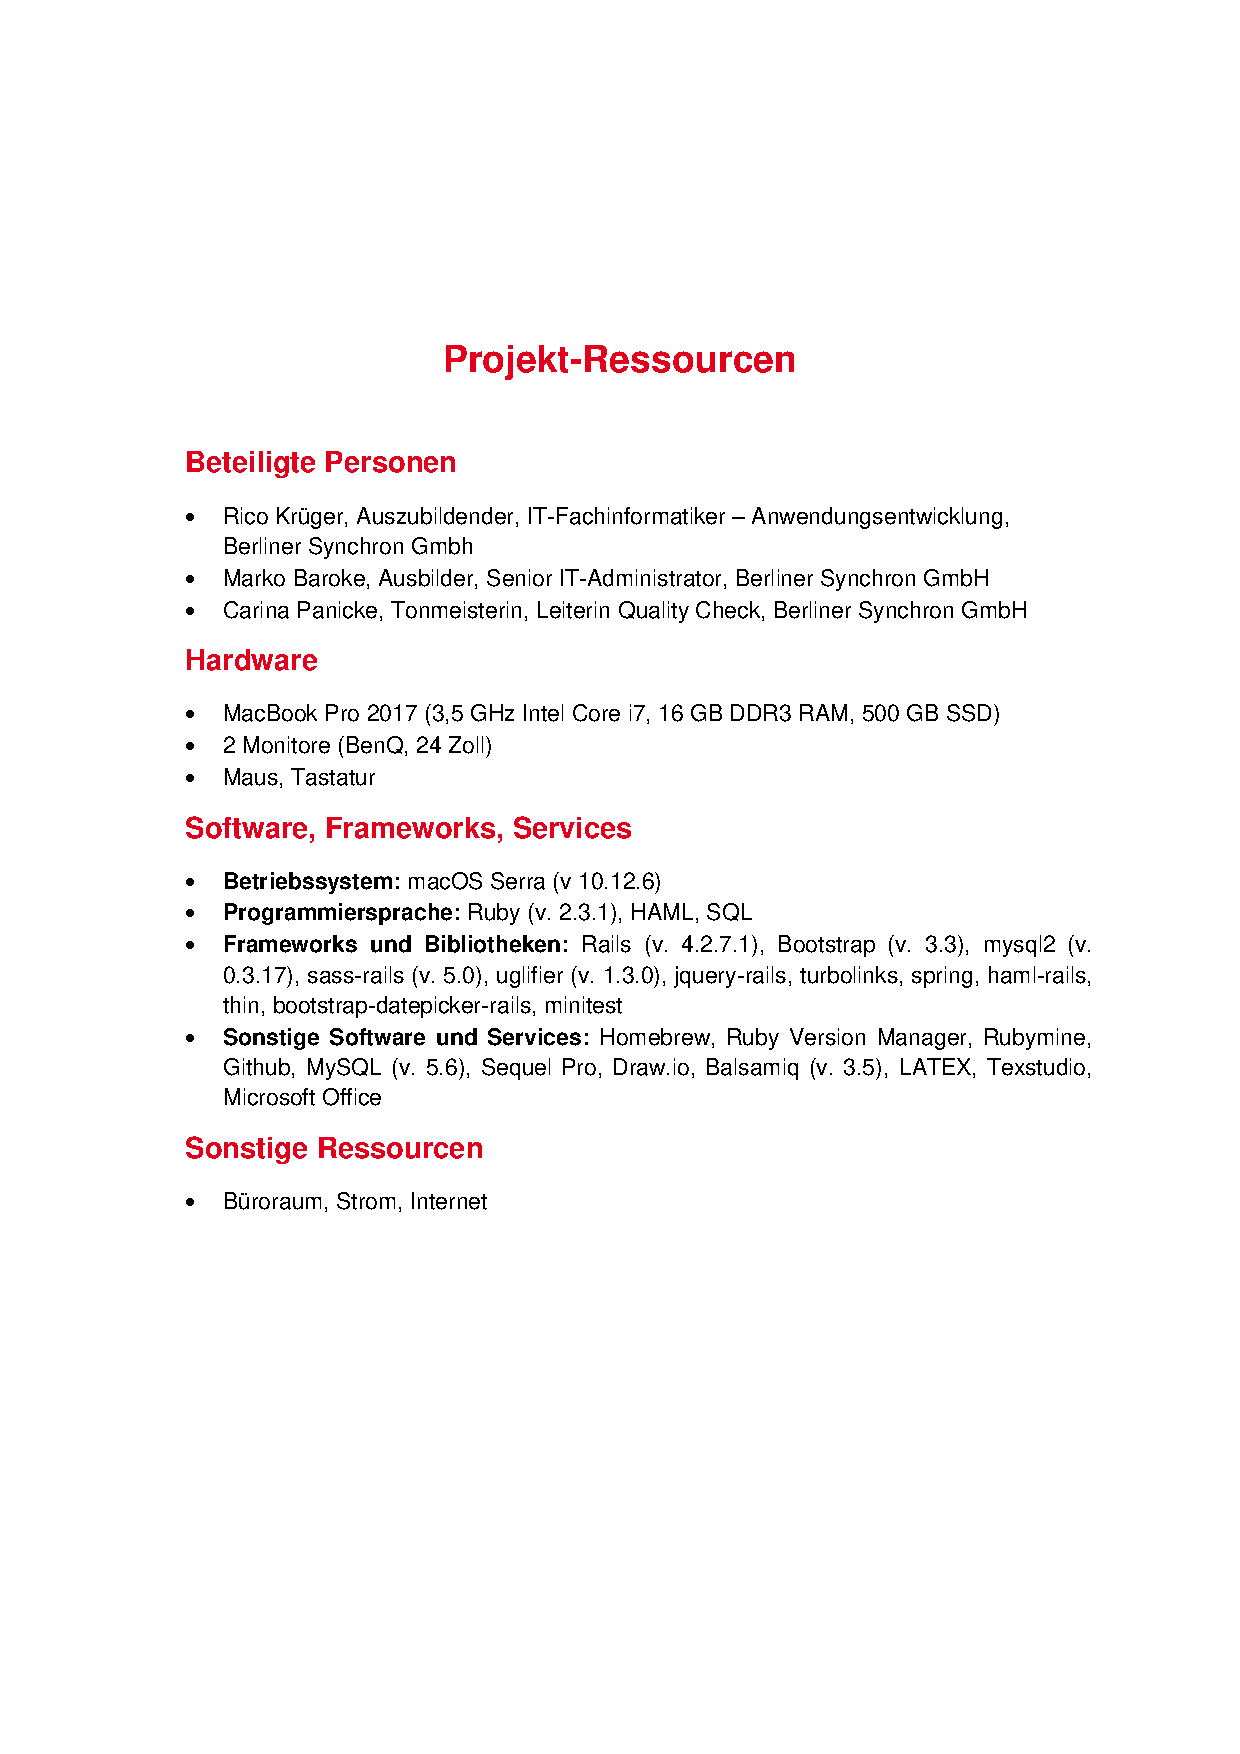
\includepdf[scale=1.0,clip,trim=0cm 0cm 0cm 0cm,offset=0 -2cm,pages={1},pagecommand={\subsection{Projekt-Ressourcen}\label{app:Ressourcen}}]{Projektressourcen.pdf}
\clearpage
\subsection{Mockups}
\label{subsec:Mockup}

\begin{figure}[htb]
\centering
\includegraphicsKeepAspectRatio{mep_index_mockup.png}{}
\caption{Mockup - Übersicht der Materialeingangsberichte}
\end{figure}

\begin{figure}[htb]
	\centering
	\includegraphicsKeepAspectRatio{mep_new_mockup.png}{}
	\caption{Mockup - Eingabeformular eines Materialeingangsberichts}
\end{figure}
\clearpage
\subsection{Datenbankentwurf}
\label{subsec:ER}

\begin{figure}[htb]
\centering
\includegraphicsKeepAspectRatio{er_model.png}{}
\caption{Entwurf der MySQL - Datenbank}
\end{figure}

\clearpage
\subsection{Testprotokoll}
\label{subsec:Testprotokoll}

\begin{figure}[htb]
	\centering
	\includegraphicsKeepAspectRatio{Testprotokoll.png}{1.0}
	\caption{Auszug aus dem Testprotokoll}
\end{figure}

\clearpage
\subsubsection{Routes.rb}
\label{app:Routes}
\lstinputlisting[language=Ruby]{Listings/routes.rb}
\subsubsection{Migration.rb}
\label{app:Migration}
\lstinputlisting[language=Ruby]{Listings/migration.rb}
\clearpage
\subsubsection{Model.rb}
\label{app:Model}
\lstinputlisting[language=Ruby]{Listings/model.rb}
\clearpage
\subsubsection{Controller.rb}
\label{app:Controller_rb}
\lstinputlisting[language=Ruby]{Listings/controller.rb}
\clearpage
\subsubsection{View.html}
\label{app:View}
\lstinputlisting[language=Ruby]{Listings/view.html.haml}
\clearpage
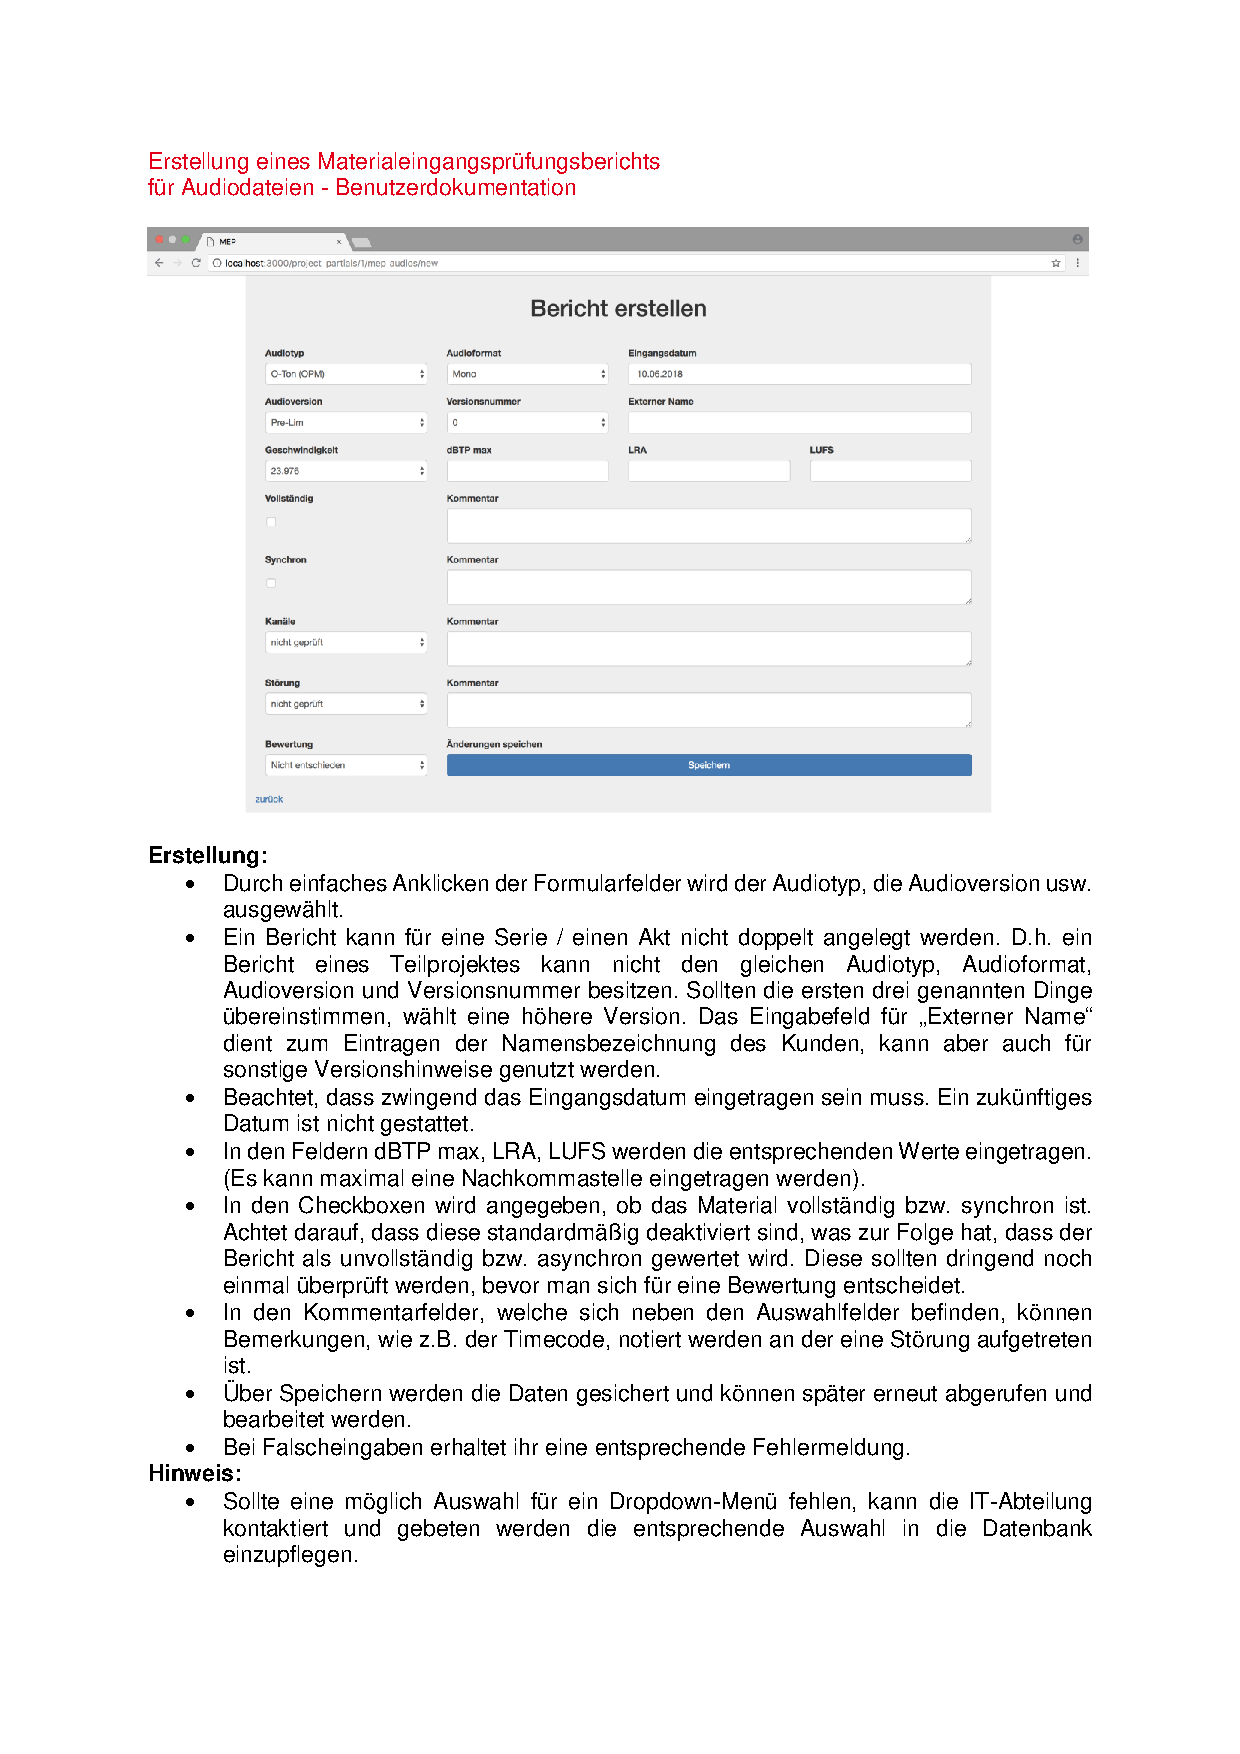
\includepdf[scale=1.0,clip,trim=0cm 0cm 0cm 0cm,offset=0 -2cm,pages={1},pagecommand={\subsection{Auszug Benutzerdokumentation}\label{app:Benutzerdokumentation}}]{Benutzerdokumentation.pdf}
%\clearpage
%\subsection{Ansicht des Eingabeformulars}
\label{subsec:Screenshot}

\begin{figure}[htb]
\centering
\includegraphicsKeepAspectRatio{mep_new_large.png}{}
\caption{Eingabeformular eines Materialeingangberichts}
\end{figure}

% \subsection{Lastenheft}
\label{app:Lastenheft}
Es folgt unser Lastenheft mit Fokus auf den Anforderungen:

Die Umsetzung muss folgende Anforderungen erfüllen: 
\begin{enumerate}[itemsep=0em,partopsep=0em,parsep=0em,topsep=0em]
\item DMZ
	\begin{enumerate}
	\item Die DMZ soll aus zwei virtuellen, zu Routern konfigurierten Linux-Distributionen bestehen, welch die Netze INSIDE, OUTSIDE und das DMZ-Netz miteinander verbinden. 
	\item Die Router sollen entsprechend des Netzplanes eingerichtet und konfiguriert werden.
	\item Die DMZ soll Zugriffe auf den Webserver erlauben, aber Zugriffe auf das INSIDE-Netz verhindern. Hierzu soll auf dem Outside-Router NAT, Portforwarding und eine Firewall laufen.
    \item Die Router sollen nur vom Client-Rechner her fernadministrierbar sein.
	\end{enumerate}
\item Client-Rechner
\begin{enumerate}
    \item Der Client-Rechner im INSIDE-Netz nutzt das Betriebssystem Windows.
    \item Der Webserver soll eine Webseite mit dem aktuellen Stand der Gruppe anzeigen.    
\end{enumerate}
\item Webserver
\begin{enumerate}
    \item Der Webserver nutzt das Betriebssystem Windows. Er wird über das Tool Mini-Webserver vom Auftraggeber bereitgestellt.
    \item Der Webserver im DMZ-Netz muss vom OUTSIDE-Netz über Port 80 erreichbar sein. Hierzu soll auf dem Outside-Router NAT und Port-Forwarding eingerichtet werden.
    \item Der Webserver soll eine Webseite mit dem aktuellen Stand der Gruppe anzeigen.    
\end{enumerate}
\item Firewall
\begin{enumerate}
    \item Die Firewall soll den Webserver in der DMZ über Port 80 erreichbar sein lassen.
    \item Die Firewall soll SSH nur vom Admin-PC zulassen.
    \item Die Firewall soll ICMP zulassen.
    \item Die Firewall soll DNS zulassen.
    \item Die Firewall soll RDP zulassen.
    \item Die Firewall soll per Script an- und ausschaltbar sein. Hierzu muss an diversen Stellen per Script die Linux-Systemkonfiguration verändert werden
\end{enumerate}
\item Sonstige Anforderungen
	\begin{enumerate}
	\item Das Projekt soll unter Berücksichtigung der von der IHK ausgegebenen Richtlinien für eine Projektdokumentation dokumentiert werden.
    \item Es soll ein logischer Netzplan in Papierform erstellt und der Dokumentation angefügt werden.
	\item Pro Person soll ein ausführliches Kompetenzportfolio erstellt werden, welches einen kritischen Überblick über unsere individuellen Kompetenzstände vor, während und nach dem Projekt liefert. Diese sollen der Dokumentation angehängt werden.
	\item Die Funktionalität der Firewall soll getestet und die Ergebnisse in zwei Testprotokollen festgehalten werden. Diese sind der Dokumentation anzuhängen.
	\end{enumerate}
\end{enumerate}


% \subsection{Pflichtenheft}
\label{app:Pflichtenheft}

Unser aus den Anforderungen des Lastenheftes erstelltes Pflichtenheft:

\begin{enumerate}[itemsep=0em,partopsep=0em,parsep=0em,topsep=0em]
\item Musskriterien % Wikipedia: für das Produkt unabdingbare Leistungen, die in jedem Fall erfüllt werden müssen
    \begin{enumerate}
    \item Das DMZ-Netz erhält die Netzmaske 172.16.9.0/24
    \item Das intere Netz erhält die Netzmaske 10.0.9.0/24
    \item Die öffentliche Schnittstelle des Outside-Router erhält die IP 192.168.200.109
    \item Der Outside-Router erhält als Standard-Gateway die IP 192.168.200.1
    \item Der Outside-Router erhält eine statische Route für das interne und DMZ-Netz
    \item Der Inside-Router erhält als Standard-Gateway das Interface des Outside-Routers, welches in die DMZ zeigt
    \item Der Webserver ist über die öffentliche IP des Outside-Routers über HTTP/S von außen erreichbar
    \item Der Webserver ist über die lokale IP 172.16.9.3 über HTTP/S aus dem internen Netzwerk erreichbar
    \item Die Router und Windows-Clients bekommen als DNS-Server die IPs 192.168.95.40 und 192.168.95.41
    \item Die Router und Windows-Clients bekommen als NTP-Server die IP 192.168.200.1
    \item Die Firewall verhindert unrechtmäßigen Datentransfer zwischen den Netzen und auf den Routern
    \item Der Admin-PC mit der IP 10.0.9.2 ist berechtigt mittels SSH auf die Router zuzugreifen	
    \end{enumerate}
\item Kannkriterien
    \begin{enumerate}
    \item Die Firewall lässt sich mit den Optionen "start" und "stop" an- bzw.\ ausschalten
    \item Die Firewall-Scripts der Router befinden sich im Verzeichnis /root/bin
    \item Die Veränderung der Firewall-Konfiguration befindet sich jeweils im Verzeichnis /var/log/firewall
    \item Der Admin-PC mit der IP 10.0.9.2 ist berechtigt mittels RDP auf den Webserver zuzugreifen
    \end{enumerate}
\end{enumerate}
	
% \clearpage

% \subsection{Netzpläne}
% \label{app:Netzplan}
% Der Netzplan unserer \ac{DMZ} in der Projektumgebung im Labor 3.1.01:
% \begin{figure}[htb]
% \centering
% \includegraphicsKeepAspectRatio{PLZNetzplanProjektumgebung.png}{0.8}
% \caption{Netzplan der \ac{DMZ} in Raum 3.1.01 (Arbeitsgruppe 9)}
% \end{figure}

% Der Netzplan unserer \ac{DMZ} in der virtualisierten Testumgebung:
% \begin{figure}[htb]
%     \centering
%     \includegraphicsKeepAspectRatio{PLZNetzplanTestumgebung.png}{0.8}
%     \caption{Netzplan der erweiterten \ac{DMZ} in unserer virtuellen Testumgebung}
% \end{figure}
% \clearpage

% \includepdf[scale=0.925,clip,trim=0cm 0cm 0cm 0cm,offset=0.7cm -1cm,landscape=true,pages={1},pagecommand={\subsection{Kompetenzportfolios}\label{app:Kompetenz}}]{Kompetenzportfolios.pdf}
% \includepdf[scale=0.95,clip,trim=0cm 0cm 0cm 0cm,offset=0.5cm -0.4cm,landscape=true,pages={2-3},pagecommand={}]{Kompetenzportfolios.pdf}
% \clearpage

% \section{Testdokumentation}
% \label{app:Test}

% \begin{table}[!ht]
    \tabelleAnhang{Systeminformation}{tab:Systeminformation}{Systeminformation.tex}
    \caption{Hardwaredetails des Testsystems}
    \label{tab:tabletestsystem}
\end{table}

\subsection{Aufbau der Testumgebung}
\label{app:testaufbau}
Die zur Umsetzung dieses Kapitels benötigten Informationen entstammen unter anderem den hilfreichen Artikeln folgender Webseiten: \cite{networkdriverhacking}

\subsubsection{Implementierung der Virtuellen Maschinen}
Im Server-Manager fügen wir über \textit{Verwalten > Rollen und Features hinzufügen} den Hyper-V-Manager hinzu indem wir dem Assistenten folgen. Dieser gestattet es virtuelle Maschinen und Netzwerke zu installieren.
Als nächstes wird eine neue virtuelle Linux (Debian 7.1)  Maschine (Generation 1) aus einem Image erstellt. Dies geschieht mit Hilfe eines Assistenten. Sie bekommt einen virtuellen Prozessor und 1 \ac{GB} Arbeitsspeicher. Des weiteren wird bei der Installation eine 5 \ac{GB} große Festplatte für die Maschine erstellt und ihr zugewiesen. Als virtuellen Switch weisen wir ihr vorläufig den Netzwerkadapter des Hosts zu. Somit besitzt unsere Linux-\ac{VM} Internet. Um sie zu installieren, startet man nun die Maschine und verbindet sich zu ihr. Danach folgt man wie gewohnt den Installationsschritten wie bei einer physischen Maschine. Danach installieren wir den \ac{NTP}-Service. Ist die Grundkonfiguration fertig, wird die Maschine ausgeschaltet.
Die Installation der Windows 7 \ac{VM} erfolgt analog zu die der Linux \ac{VM}. Wir vergeben jedoch 4 \ac{GB} \ac{RAM} und erstellen eine mindestens 30 \ac{GB} große virtuelle Festplatte. Nach der Installation wird die Firewall wie in \nameref{sec:Implementierungsphase} eingerichtet. Zusätzlich werden noch nützliche Software wie putty oder winscp heruntergeladen.
Nach der Grundkonfiguration der beiden \ac{VM}s können diese nun dupliziert werden. Dazu muss man die virtuelle Maschine erst exportieren, um sie danach wieder zu importieren. Beim Import sollte man darauf achten, dass man \textit{eine neue eindeutige \ac{ID} } erstellt. Nachdem starten der importierten Maschine wird als erstes der Hostname geändert, um sie von der Originalen zu unterscheiden und um \ac{DNS}-Konflikte zu vermeiden.

\subsubsection{Implementierung des virtuellen Netzwerkes}
Virtuelle Netzwerke werden über das Hinzufügen virtueller Switche an den Netzwerkadaptern der virtuellen Maschine erstellt. Auf diesen lassen sich auch \ac{VLAN}s einrichten.
Die Installation eines solchen Switch wird ebenfalls vom Hyper-V-Manager mit einem Assistenten bereitgestellt. Für Testzwecke werden 2 \textit{private} Switche erstellt, da diese die direkte Kommunikation mit dem Host unterbinden und somit nicht die Router umgangen werden. Diese erhalten den Namen \ac{DMZ}- \bzw \ac{LAN}-Switch. Ein \textit{öffentlicher} Switch ist bereits vorhanden. Mit diesem ist der physische Netzwerkadapter des Hosts verbunden. Diese werden dann den \ac{VM}s entsprechend des \nameref{app:Netzplan}s zugeordnet. Für die Linux-\ac{VM}s, die als Router fungieren, muss \evtl noch ein zweiter Netzwerkadapter hinzugefügt werden. Nun können die Router und Clients (\text{Siehe Bild und Implementierung}) konfiguriert werden.

\subsubsection{Implementierung des \ac{DNS}-Servers}
Der \ac{DNS}-Server wird ebenfalls über den Server-Manager (unter \textit{Rollen und Features hinzufügen}) installiert. Diesen kann man nun über den \ac{DNS}-Manager verwalten. Es genügt eine \textit{Forward-Lookup}-Zone zu erstellen. Als Zonennamen wählen wir \textit{fritz.box} da bereits das Standard-Gateway darauf verweist. Dies ist die Domäne bzw. das \ac{DNS}-Suffix. Dieses Suffix wird auf den Windows-\ac{VM}s in den \ac{IP}v4-Einstellungen des Netzwerkadapters nachgetragen. Auf den Linux-\ac{VM}s tragen wir dies zusätzlich in die \verb+/etc/resolv.conf+ vor unserem \ac{DNS}-Server ein. \textbf{siehe resolv.conf oder selber schreiben]
Über den \ac{DNS}-Manager werden im Anschluss noch in der Zone \textit{fritz.box} unsere \ac{VM}s (A-Record) mit Namen und \ac{IP}-Adressen eingetragen. \textbf Siehe \ac{DNS}Manager.png}.

\subsubsection{Testen der Firewall}
Nachdem das Firewall-Script auf die Router kopiert und die \ac{DNS}-Server angepasst wurden, kann mit den Tests begonnen und die Firewall ggf.\ angepasst werden. Dazu speichern wir den Verlauf der erstellten Regeln als Log-Ausgabe in \verb+/var/log/firewall/firewallConfig+ ab. Die Ergebnisse unserer Tests finden sich als Übersicht in den folgenden Tabellen der Testprotokolle:


% Testprotokolle
\subsubsection{Testprotokolle}
\label{app:Testprotokolle}
% Description
\clearpage

% tables created with: http://www.tablesgenerator.com/latex_tables
% Please add the following required packages to your document preamble:
% \usepackage{graphicx}
% \usepackage[table,xcdraw]{xcolor}
% If you use beamer only pass "xcolor=table" option, i.e. \documentclass[xcolor=table]{beamer}
\begin{table}[!ht]
    \resizebox{\textwidth}{!}{%
        \begin{tabular}{llllll}
            \rowcolor[HTML]{009BA7} 
            \textbf{Service} & \textbf{Command} & \textbf{Source-IP} & \textbf{Destination-IP} & \textbf{Soll} & \textbf{Ist} \\
            ICMP & ping & 10.0.9.2 & 10.0.9.1 & ja & ja \\
            \rowcolor[HTML]{EFEFEF} 
            ICMP & ping & 10.0.9.3 & 10.0.9.1 & ja & ja \\
            ICMP & ping & 10.0.9.2 & 172.16.9.1 & ja & ja \\
            \rowcolor[HTML]{EFEFEF} 
            ICMP & ping & 10.0.9.3 & 172.16.9.1 & ja & ja \\
            ICMP & ping & 172.16.9.3 & 172.16.9.1 & ja & ja \\
            \rowcolor[HTML]{EFEFEF} 
            ICMP & ping & 172.16.9.3 & 172.16.9.2 & ja & ja \\
            ICMP & ping & 10.0.9.3 & 192.168.200.10 & ja & ja \\
            \rowcolor[HTML]{EFEFEF} 
            ICMP & ping & 192.168.200.10 & 10.0.9.3 & ja & ja \\
            ICMP & ping & 192.168.200.10 & 172.16.9.3 & ja & ja \\
            \rowcolor[HTML]{EFEFEF} 
            ICMP & ping & 192.168.200.10 & 192.168.200.109 & ja & ja \\
            ICMP & ping & 10.0.9.3 & 8.8.8.8 & ja & ja \\
            \rowcolor[HTML]{EFEFEF} 
            HTTP & http://172.16.9.3 & 192.168.200.10 & 192.168.200.109 & ja & ja \\
            HTTP & http://172.16.9.3 & 192.168.200.10 & 172.16.9.3 & ja & ja \\
            \rowcolor[HTML]{EFEFEF} 
            HTTP & http://172.16.9.3 & 10.0.9.3 & 192.168.200.109 & ja & ja \\
            HTTP & http://172.16.9.3 & 10.0.9.3 & 172.16.9.3 & ja & ja \\
            \rowcolor[HTML]{EFEFEF} 
            NTP & w32tm /stripchart /computer:192.168.200.1 & 10.0.9.2 & 192.168.200.1 & ja & ja \\
            NTP & w32tm /stripchart /computer:192.168.200.1 & 172.16.9.3 & 192.168.200.1 & ja & ja \\
            \rowcolor[HTML]{EFEFEF} 
            NTP & ntpq -p & 192.168.200.109 & 192.168.200.1 & ja & ja \\
            RDP & mstsc.exe & 10.0.9.2 & 172.16.9.3 & ja & ja \\
            \rowcolor[HTML]{EFEFEF} 
            RDP & mstsc.exe & 10.0.9.3 & 172.16.9.3 & ja & ja \\
            SSH & putty & 10.0.9.2 & 10.0.9.1 & ja & ja \\
            \rowcolor[HTML]{EFEFEF} 
            SSH & putty & 10.0.9.2 & 172.16.9.1 & ja & ja \\
            SSH & putty & 10.0.9.3 & 10.0.9.1 & ja & ja \\
            \rowcolor[HTML]{EFEFEF} 
            SSH & putty & 10.0.9.3 & 172.16.9.1 & ja & ja \\
            SSH & putty & 172.16.9.3 & 172.16.9.1 & ja & ja \\
            \rowcolor[HTML]{EFEFEF} 
            SSH & putty & 172.16.9.3 & 172.16.9.2 & ja & ja \\
            DNS & nslookup 172.16.9.1 & 10.0.9.3 & 192.168.200.10 & ja & ja \\
            \rowcolor[HTML]{EFEFEF} 
            DNS & nslookup Inside-Router & 172.16.9.3 & 192.168.200.10 & ja & ja \\
            DNS & nslookup 10.0.9.1 & 172.16.9.2 & 192.168.200.10 & ja & ja \\
            \rowcolor[HTML]{EFEFEF} 
            DNS & nslookup Client-PC & 192.168.200.109 & 192.168.200.10 & ja & ja
        \end{tabular}%
    }
    \caption{Aus - Aus}
    \label{tab:ausaus}
\end{table}

% Please add the following required packages to your document preamble:
% \usepackage{graphicx}
% \usepackage[table,xcdraw]{xcolor}
% If you use beamer only pass "xcolor=table" option, i.e. \documentclass[xcolor=table]{beamer}
\begin{table}[!ht]
    \resizebox{\textwidth}{!}{%
        \begin{tabular}{llllll}
            \rowcolor[HTML]{009BA7} 
            \textbf{Service} & \textbf{Command} & \textbf{Source-IP} & \textbf{Destination-IP} & \textbf{Soll} & \textbf{Ist} \\
            ICMP & ping & 10.0.9.2 & 10.0.9.1 & ja & ja \\
            \rowcolor[HTML]{EFEFEF} 
            ICMP & ping & 10.0.9.3 & 10.0.9.1 & nein & nein \\
            ICMP & ping & 10.0.9.2 & 172.16.9.1 & ja & ja \\
            \rowcolor[HTML]{EFEFEF} 
            ICMP & ping & 10.0.9.3 & 172.16.9.1 & nein & nein \\
            ICMP & ping & 172.16.9.3 & 172.16.9.1 & ja & ja \\
            \rowcolor[HTML]{EFEFEF} 
            ICMP & ping & 172.16.9.3 & 172.16.9.2 & nein & nein \\
            ICMP & ping & 10.0.9.3 & 192.168.200.10 & ja & ja \\
            \rowcolor[HTML]{EFEFEF} 
            ICMP & ping & 192.168.200.10 & 10.0.9.3 & nein & nein \\
            ICMP & ping & 192.168.200.10 & 172.16.9.3 & ja & ja \\
            \rowcolor[HTML]{EFEFEF} 
            ICMP & ping & 192.168.200.10 & 192.168.200.109 & ja & ja \\
            ICMP & ping & 10.0.9.3 & 8.8.8.8 & ja & ja \\
            \rowcolor[HTML]{EFEFEF} 
            HTTP & http://172.16.9.3 & 192.168.200.10 & 192.168.200.109 & ja & ja \\
            HTTP & http://172.16.9.3 & 192.168.200.10 & 172.16.9.3 & ja & ja \\
            \rowcolor[HTML]{EFEFEF} 
            HTTP & http://172.16.9.3 & 10.0.9.3 & 192.168.200.109 & nein & nein \\
            HTTP & http://172.16.9.3 & 10.0.9.3 & 172.16.9.3 & ja & ja \\
            \rowcolor[HTML]{EFEFEF} 
            NTP & w32tm /stripchart /computer:192.168.200.1 & 10.0.9.2 & 192.168.200.1 & ja & ja \\
            NTP & w32tm /stripchart /computer:192.168.200.1 & 172.16.9.3 & 192.168.200.1 & ja & ja \\
            \rowcolor[HTML]{EFEFEF} 
            NTP & ntpq -p & 192.168.200.109 & 192.168.200.1 & ja & ja \\
            RDP & mstsc.exe & 10.0.9.2 & 172.16.9.3 & ja & ja \\
            \rowcolor[HTML]{EFEFEF} 
            RDP & mstsc.exe & 10.0.9.3 & 172.16.9.3 & nein & nein \\
            SSH & putty & 10.0.9.2 & 10.0.9.1 & ja & ja \\
            \rowcolor[HTML]{EFEFEF} 
            SSH & putty & 10.0.9.2 & 172.16.9.1 & ja & ja \\
            SSH & putty & 10.0.9.3 & 10.0.9.1 & nein & nein \\
            \rowcolor[HTML]{EFEFEF} 
            SSH & putty & 10.0.9.3 & 172.16.9.1 & ja & ja \\
            SSH & putty & 172.16.9.3 & 172.16.9.1 & ja & ja \\
            \rowcolor[HTML]{EFEFEF} 
            SSH & putty & 172.16.9.3 & 172.16.9.2 & nein & nein \\
            DNS & nslookup 172.16.9.1 & 10.0.9.3 & 192.168.200.10 & ja & ja \\
            \rowcolor[HTML]{EFEFEF} 
            DNS & nslookup Inside-Router & 172.16.9.3 & 192.168.200.10 & ja & ja \\
            DNS & nslookup 10.0.9.1 & 172.16.9.2 & 192.168.200.10 & ja & ja \\
            \rowcolor[HTML]{EFEFEF} 
            DNS & nslookup Client-PC & 192.168.200.109 & 192.168.200.10 & ja & ja
        \end{tabular}%
    }
    \caption{Aus - An}
    \label{tab:ausan}
\end{table}

% Please add the following required packages to your document preamble:
% \usepackage{graphicx}
% \usepackage[table,xcdraw]{xcolor}
% If you use beamer only pass "xcolor=table" option, i.e. \documentclass[xcolor=table]{beamer}
\begin{table}[!ht]
    \resizebox{\textwidth}{!}{%
        \begin{tabular}{llllll}
            \rowcolor[HTML]{009BA7} 
            \textbf{Service} & \textbf{Command} & \textbf{Source-IP} & \textbf{Destination-IP} & \textbf{Soll} & \textbf{Ist} \\
            ICMP & ping & 10.0.9.2 & 10.0.9.1 & ja & ja \\
            \rowcolor[HTML]{EFEFEF} 
            ICMP & ping & 10.0.9.3 & 10.0.9.1 & ja & ja \\
            ICMP & ping & 10.0.9.2 & 172.16.9.1 & ja & ja \\
            \rowcolor[HTML]{EFEFEF} 
            ICMP & ping & 10.0.9.3 & 172.16.9.1 & nein & nein \\
            ICMP & ping & 172.16.9.3 & 172.16.9.1 & nein & nein \\
            \rowcolor[HTML]{EFEFEF} 
            ICMP & ping & 172.16.9.3 & 172.16.9.2 & ja & ja \\
            ICMP & ping & 10.0.9.3 & 192.168.200.10 & ja & ja \\
            \rowcolor[HTML]{EFEFEF} 
            ICMP & ping & 192.168.200.10 & 10.0.9.3 & nein & nein \\
            ICMP & ping & 192.168.200.10 & 172.16.9.3 & nein & nein \\
            \rowcolor[HTML]{EFEFEF} 
            ICMP & ping & 192.168.200.10 & 192.168.200.109 & nein & nein \\
            ICMP & ping & 10.0.9.3 & 8.8.8.8 & ja & ja \\
            \rowcolor[HTML]{EFEFEF} 
            HTTP & http://172.16.9.3 & 192.168.200.10 & 192.168.200.109 & ja & ja \\
            HTTP & http://172.16.9.3 & 192.168.200.10 & 172.16.9.3 & ja & ja \\
            \rowcolor[HTML]{EFEFEF} 
            HTTP & http://172.16.9.3 & 10.0.9.3 & 192.168.200.109 & nein & nein \\
            HTTP & http://172.16.9.3 & 10.0.9.3 & 172.16.9.3 & ja & ja \\
            \rowcolor[HTML]{EFEFEF} 
            NTP & w32tm /stripchart /computer:192.168.200.1 & 10.0.9.2 & 192.168.200.1 & ja & ja \\
            NTP & w32tm /stripchart /computer:192.168.200.1 & 172.16.9.3 & 192.168.200.1 & ja & ja \\
            \rowcolor[HTML]{EFEFEF} 
            NTP & ntpq -p & 192.168.200.109 & 192.168.200.1 & ja & ja \\
            RDP & mstsc.exe & 10.0.9.2 & 172.16.9.3 & ja & ja \\
            \rowcolor[HTML]{EFEFEF} 
            RDP & mstsc.exe & 10.0.9.3 & 172.16.9.3 & nein & nein \\
            SSH & putty & 10.0.9.2 & 10.0.9.1 & ja & ja \\
            \rowcolor[HTML]{EFEFEF} 
            SSH & putty & 10.0.9.2 & 172.16.9.1 & ja & ja \\
            SSH & putty & 10.0.9.3 & 10.0.9.1 & ja & ja \\
            \rowcolor[HTML]{EFEFEF} 
            SSH & putty & 10.0.9.3 & 172.16.9.1 & ja & ja \\
            SSH & putty & 172.16.9.3 & 172.16.9.1 & nein & nein \\
            \rowcolor[HTML]{EFEFEF} 
            SSH & putty & 172.16.9.3 & 172.16.9.2 & ja & ja \\
            DNS & nslookup 172.16.9.1 & 10.0.9.3 & 192.168.200.10 & ja & ja \\
            \rowcolor[HTML]{EFEFEF} 
            DNS & nslookup Inside-Router & 172.16.9.3 & 192.168.200.10 & ja & ja \\
            DNS & nslookup 10.0.9.1 & 172.16.9.2 & 192.168.200.10 & ja & ja \\
            \rowcolor[HTML]{EFEFEF} 
            DNS & nslookup Client-PC & 192.168.200.109 & 192.168.200.10 & ja & ja
        \end{tabular}%
    }
    \caption{An - Aus}
    \label{tab:anaus}
\end{table}

% Please add the following required packages to your document preamble:
% \usepackage{graphicx}
% \usepackage[table,xcdraw]{xcolor}
% If you use beamer only pass "xcolor=table" option, i.e. \documentclass[xcolor=table]{beamer}
\begin{table}[!ht]
    \resizebox{\textwidth}{!}{%
        \begin{tabular}{llllll}
            \rowcolor[HTML]{009BA7} 
            \textbf{Service} & \textbf{Command} & \textbf{Source-IP} & \textbf{Destination-IP} & \textbf{Soll} & \textbf{Ist} \\
            ICMP & ping & 10.0.9.2 & 10.0.9.1 & ja & ja \\
            \rowcolor[HTML]{EFEFEF} 
            ICMP & ping & 10.0.9.3 & 10.0.9.1 & ja & ja \\
            ICMP & ping & 10.0.9.2 & 172.16.9.1 & ja & ja \\
            \rowcolor[HTML]{EFEFEF} 
            ICMP & ping & 10.0.9.3 & 172.16.9.1 & nein & nein \\
            ICMP & ping & 172.16.9.3 & 172.16.9.1 & nein & nein \\
            \rowcolor[HTML]{EFEFEF} 
            ICMP & ping & 172.16.9.3 & 172.16.9.2 & ja & ja \\
            ICMP & ping & 10.0.9.3 & 192.168.200.10 & ja & ja \\
            \rowcolor[HTML]{EFEFEF} 
            ICMP & ping & 192.168.200.10 & 10.0.9.3 & nein & nein \\
            ICMP & ping & 192.168.200.10 & 172.16.9.3 & nein & nein \\
            \rowcolor[HTML]{EFEFEF} 
            ICMP & ping & 192.168.200.10 & 192.168.200.109 & nein & nein \\
            ICMP & ping & 10.0.9.3 & 8.8.8.8 & ja & ja \\
            \rowcolor[HTML]{EFEFEF} 
            HTTP & http://172.16.9.3 & 192.168.200.10 & 192.168.200.109 & ja & ja \\
            HTTP & http://172.16.9.3 & 192.168.200.10 & 172.16.9.3 & ja & ja \\
            \rowcolor[HTML]{EFEFEF} 
            HTTP & http://172.16.9.3 & 10.0.9.3 & 192.168.200.109 & nein & nein \\
            HTTP & http://172.16.9.3 & 10.0.9.3 & 172.16.9.3 & ja & ja \\
            \rowcolor[HTML]{EFEFEF} 
            NTP & w32tm /stripchart /computer:192.168.200.1 & 10.0.9.2 & 192.168.200.1 & ja & ja \\
            NTP & w32tm /stripchart /computer:192.168.200.1 & 172.16.9.3 & 192.168.200.1 & ja & ja \\
            \rowcolor[HTML]{EFEFEF} 
            NTP & ntpq -p & 192.168.200.109 & 192.168.200.1 & ja & ja \\
            RDP & mstsc.exe & 10.0.9.2 & 172.16.9.3 & ja & ja \\
            \rowcolor[HTML]{EFEFEF} 
            RDP & mstsc.exe & 10.0.9.3 & 172.16.9.3 & nein & nein \\
            SSH & putty & 10.0.9.2 & 10.0.9.1 & ja & ja \\
            \rowcolor[HTML]{EFEFEF} 
            SSH & putty & 10.0.9.2 & 172.16.9.1 & ja & ja \\
            SSH & putty & 10.0.9.3 & 10.0.9.1 & ja & ja \\
            \rowcolor[HTML]{EFEFEF} 
            SSH & putty & 10.0.9.3 & 172.16.9.1 & ja & ja \\
            SSH & putty & 172.16.9.3 & 172.16.9.1 & nein & nein \\
            \rowcolor[HTML]{EFEFEF} 
            SSH & putty & 172.16.9.3 & 172.16.9.2 & ja & ja \\
            DNS & nslookup 172.16.9.1 & 10.0.9.3 & 192.168.200.10 & ja & ja \\
            \rowcolor[HTML]{EFEFEF} 
            DNS & nslookup Inside-Router & 172.16.9.3 & 192.168.200.10 & ja & ja \\
            DNS & nslookup 10.0.9.1 & 172.16.9.2 & 192.168.200.10 & ja & ja \\
            \rowcolor[HTML]{EFEFEF} 
            DNS & nslookup Client-PC & 192.168.200.109 & 192.168.200.10 & ja & ja
        \end{tabular}%
    }
    \caption{An - An}
    \label{tab:anan}
\end{table}
\clearpage

\subsection{Firewall-Skripte}
\label{app:Firewall}

\subsubsection{firewall.sh (auf dem Outside-Router)}
\label{app:Firewall-Outside}
\lstinputlisting[language=sh]{Listings/outside/firewall.sh}

\subsubsection{firewall.sh (auf dem Inside-Router)}
\label{app:Firewall-Inside}
\lstinputlisting[language=sh]{Listings/inside/firewall.sh}




\end{document}
